\documentclass[12pt]{article}
\usepackage{colortbl}
\usepackage{tabularx}
\usepackage{longtable}
\usepackage{comment}
\usepackage{amsmath}
\usepackage{amssymb}
\usepackage{nccmath}
\usepackage{multirow}
%\usepackage{mathtools}
\usepackage{geometry}
\usepackage{booktabs}
\usepackage{xr}
\usepackage{enumitem}
\usepackage{siunitx}
\usepackage{graphicx}
\usepackage{caption}

\definecolor{AFB}{rgb}{0.36, 0.54, 0.66}
\definecolor{Brass}{rgb}{0.71, 0.65, 0.26}
\definecolor{Amethyst}{rgb}{0.6, 0.4, 0.8}

\usepackage{xr}
\usepackage{hyperref}

\hypersetup{
    bookmarks=true,         % show bookmarks bar?
      colorlinks=true,       % false: boxed links; true: colored links
    linkcolor=red,          % color of internal links (change box
                            % color with linkbordercolor)
    citecolor=green,        % color of links to bibliography
    filecolor=magenta,      % color of file links
    urlcolor=cyan           % color of external links
}
\newcommand{\NN}[1]{{\color{red}#1}}
\newcommand{\WSS}[1]{{\color{blue}#1}}

%% Comments
\newif\ifcomments\commentstrue

\ifcomments
\newcommand{\authornote}[3]{\textcolor{#1}{[#3 ---#2]}}
\newcommand{\todo}[1]{\textcolor{red}{[TODO: #1]}}
\else
\newcommand{\authornote}[3]{}
\newcommand{\todo}[1]{}
\fi

\newcommand{\wss}[1]{\authornote{magenta}{SS}{#1}}
\newcommand{\hf}[1]{\authornote{cyan}{HF}{#1}}
\newcommand{\cjl}[1]{\authornote{green}{CL}{#1}}

\newcommand{\progname}{SSP}

\newcommand{\colAwidth}{0.13\textwidth}
\newcommand{\colBwidth}{0.82\textwidth}
\newcommand{\colCwidth}{0.1\textwidth}
\newcommand{\colDwidth}{0.05\textwidth}
\newcommand{\colEwidth}{0.8\textwidth}
\newcommand{\colFwidth}{0.17\textwidth}
\newcommand{\colGwidth}{0.5\textwidth}
\newcommand{\colHwidth}{0.28\textwidth}
\newcounter{assumpnum} %Assumption Number
\newcommand{\atheassumpnum}{A\theassumpnum}
\newcommand{\aref}[1]{A\ref{#1}}
\newcounter{goalnum} %Goal Number
\newcommand{\gthegoalnum}{GS\thegoalnum}
\newcommand{\gsref}[1]{GS\ref{#1}}
\newcounter{theorynum} %Theory Number
\newcommand{\tthetheorynum}{T\thetheorynum}
\newcommand{\tref}[1]{T\ref{#1}}
\renewcommand{\arraystretch}{1}
\newcounter{instnum} %Instance Number
\newcommand{\itheinstnum}{IM\theinstnum}
\newcommand{\iref}[1]{IM\ref{#1}}
\newcounter{datadefnum} %Datadefinition Number
\newcommand{\ddthedatadefnum}{DD\thedatadefnum}
\newcommand{\ddref}[1]{DD\ref{#1}}
\newcounter{defnum} %Definition Number
\newcommand{\dthedefnum}{GD\thedefnum}
\newcommand{\dref}[1]{GD\ref{#1}}
\newcounter{reqnum} %Requirement Number
\newcommand{\rthereqnum}{R\thereqnum}
\newcommand{\rref}[1]{R\ref{#1}}
\newcounter{lcnum} %Likely change number
\newcommand{\lthelcnum}{LC\thelcnum}
\newcommand{\lcref}[1]{LC\ref{#1}}
\newcounter{ucnum} %Unlikely change number
\newcommand{\ltheucnum}{UC\theucnum}
\newcommand{\ucref}[1]{UC\ref{#1}}
\newcounter{fnum} %Figure number
\newcommand{\fthefnum}{Fig\thefnum}
\newcommand{\fref}[1]{Fig \ref{#1}}
\newcounter{tablenum} %Table number
\newcommand{\tablethetablenum}{Table\thetablenum}
\newcommand{\tableref}[1]{Table\ref{#1}}

\newcommand{\forceindent}{\parindent=1em\indent\parindent=0pt\relax}

%\oddsidemargin -1000mm
%\evensidemargin -1000mm
%\textwidth 160mm
%\textheight 300mm
\newgeometry{margin=2cm}

\externaldocument[MIS-]{MIS_SSP}
\externaldocument[MG-]{MG_SSP}

\begin{document}

\title{Software Requirements Specification for Slope Stability Analysis}
\author{Henry Frankis\\McMaster University}
\date{\today}
	
\maketitle
\tableofcontents

\section{Reference Material}
This section records information for easy reference.
\subsection{Table of Units}

The unit system used throughout is SI (Syst\`{e}me International d'Unit\'{e}s). In
 addition to the basic units, several derived units are also used. For each unit, the table
 lists the symbol, a description and the SI name.
\newline

\renewcommand{\arraystretch}{1.2}
\setlength{\tabcolsep}{20pt}
\begin{tabular}{  l  l  l  }
\hline
\textbf{Physical Property} & \textbf{Name} & \textbf{Symbol} \\
\hline
force & Newton & \si{\newton} \\
length & meter & \si{\meter}  \\
pressure & Pascal & $\si{\pascal}=\si{\newton\per\square\meter}$ \\
angle & degree & \si{\degree}  \\
\hline
\end{tabular}
\renewcommand{\arraystretch}{1}


\subsection{Table of Symbols}


The table that follows summarizes the symbols used in this document along with their units. 
Throughout the document, values with a subscript $i$ implies that the value will be taken at
 and analyzed at a slice or slice interface composing the total slip mass.

\renewcommand{\arraystretch}{1.6}
\setlength{\tabcolsep}{20pt}
\begin{longtable}{  l  l  p{8.5cm}  }
\hline
\textbf{Symbol} & \textbf{Unit} & \textbf{Description} \\
\hline
$\{{x_{cs}}{,y_{cs}}\}$ & \si{\meter}& The Set of X and Y Coordinates: describe the vertices of the critical slip surface 
\\
$(x,y)$ & \si{\meter}& Cartesian Position Coordinates: y is considered parallel to the direction of the force of gravity and x is considered perpendicular to y
\\
$a$ & \si{\meter}& Constant: FIXME: missing description
\\
$A$ & \si{\meter}& Constant: FIXME: missing description
\\
$b$ & \si{\meter}& Base Width of a Slice: in the x-ordinate direction only for slice index i
\\
$c'$ & \si{\pascal} & Effective Cohesion: internal pressure that sticks particles of soil together 
\\
${C1_{i}}$ &  N\si{\meter}&Interslice Normal Force Function: the normal force at the interslice interface for slice i
\\
${C2_{i}}$ &  N\si{\meter}&Interslice Shear Force Function: the shear force at the interslice interface for slice i
\\
$E$ & \si{\pascal} & Elastic Modulus: The ratio of the stress exerted on a body to the resulting strain.
\\
$F$ &\si{\newton} & Force: An interaction that tends to produce change in the motion of an object 
\\
${F_{x}}$ & \si{\newton} &$x$-component of the net force
\\
${F_{y}}$ & \si{\newton} &$y$-component of the net force
\\
$f$ & & Scaling Function: magnitude of interslice forces as a function of the x coordinate for interslice index i; can be constant or a half-sine
\\
$FS$ & &Factor of Safety: The global stability of a surface in a slope  
\\
${FS_{Loc,i}}$ & & Local Factor of Safety: for slice index i  
\\
$G$ & \si{\newton} & Interslice Normal Force: exerted between adjacent slices for interslice index i
\\
$H$ & \si{\newton} &Interslice Water Force: exerted in the x-ordinate direction between adjacent slices for interslice index i
\\
$\Delta{}H$ & \si{\newton} & Difference Between Interslice Forces: exerted in the x-ordinate direction between adjacent slices for interslice index i
\\
$h$ &  \si{\meter}&Midpoint Height: distance from the slip base to the slope surface in a vertical line from the midpoint of the slice for slice index i
\\
$i$ & & Index: used to show a quantity applies to only one slice 
\\
${K_{bA}}$ &\si{\pascal\per\meter} & Effective Base Stiffness a: for rotated coordinates of a slice base surface, for slice index i
\\
${K_{bB}}$ &\si{\pascal\per\meter} & Effective Base Stiffness a: for rotated coordinates of a slice base surface, for slice index i
\\
$K$ &  \si{\pascal\per\meter} &Stiffness: The extent a body resists strain.
\\
${K_{bn}}$ & \si{\pascal\per\meter} & Normal Stiffness: for a slice base surface, without length adjustment for slice index i
\\
${K_{bt}}$ & \si{\pascal\per\meter} & Shear Stiffness: for a slice base surface, without length adjustment for slice index i
\\
${K_{c}}$ & & Earthquake Load Factor: proportionality factor of force that weight pushes outwards; caused by seismic earth movements 
\\
${K_{no}}$ &\si{\pascal\per\meter} & Normal Stiffness: residual strength
\\
${K_{sn}}$ &\si{\pascal\per\meter} & Normal Stiffness: for an interslice surface, without length adjustment for interslice index i
\\
${K_{st}}$ & \si{\pascal\per\meter} & Shear Stiffness: for interslice surface, without length adjustment for interslice index i
\\
${K_{tr}}$ &\si{\pascal\per\meter} & Shear Stiffness: residual strength
\\
$M$ & N  \si{\meter}& Moment: a measure of the tendency of a body to rotate about a specific point or axis
\\
$N$ & \si{\newton} & Normal Force: total reactive force for a soil surface subject to a body resting on it
\\
$N'$ &\si{\newton} & Effective Normal Force: for a soil surface, subtracting pore water reactive force from total reactive force 
\\
$n$ & & Number of Slices: the slip mass has been divided into  
\\
$N*$ &\si{\newton} & Effective Normal Force: for a soil surface, without the influence of interslice forces
\\
$p$ & \si{\pascal} & Pressure: A force exerted over an area
\\
$P$ & \si{\newton} & Resistive Shear Force: Mohr Coulomb frictional force that describes the limit of mobilized shear force the slice i can withstand before failure
\\
$Q$ & \si{\newton} & Imposed Surface Load: a downward force acting into the surface from midpoint of slice i
\\
$R$ & \si{\newton} & Resistive Shear Force: without the influence of interslice forces for slice index i
\\
$S$ & \si{\newton} & Mobilized Shear Force: for slice index i
\\
$s$ &\si{\pascal} & Mobilized Shear Stress: acting on the base of a slice
\\
$T$ & \si{\newton} & Mobilized Shear Force: without the influence of interslice forces for slice index i
\\
${U_{b}}$ & \si{\newton} & Base Hydrostatic Force: from water pressure within the slice for slice index i
\\
${U_{t}}$ & \si{\newton} & Surface Hydrostatic Force: from water pressure acting into the slice from standing water on the slope surface for slice index i
\\
$u$ & & Local Index: used as a bound variable index in calculations
\\
$v$ &  &Local Index: used as a bound variable index in calculations
\\
$W$ & \si{\newton} &Weight: downward force caused by gravity on slice i
\\
$x$ & \si{\meter}& X Ordinate: refers to either slice i midpoint, or slice interface i
\\
${x_{slip}}$ &  \si{\meter}&X Ordinate: distance of the slip surface at i, refers to either slice i midpoint, or slice interface i
\\
${x_{us}}$ &  \si{\meter}&X Ordinate: distance of the edge of the slope at i, refers to either slice i midpoint, or slice interface i
\\
$X$ & \si{\newton} & Interslice Shear Force: exerted between adjacent slices for interslice index i
\\
${y_{slip}}$ & \si{\meter}& Y Ordinate: height of the slip surface at i, refers to either slice i midpoint, or slice interface i 
\\
${y_{us}}$ &  \si{\meter}&Y Ordinate: height of the top of the slope at i, refers to either slice i midpoint, or slice interface i 
\\
${y_{wt}}$ &  \si{\meter}&Y Ordinate: height of the water table at i, refers to either slice i midpoint, or slice interface i 
\\
$y$ &  \si{\meter}&Y Ordinate: refers to either slice i midpoint, or slice interface i 
\\
$z$ & \si{\meter}& Center of Slice Height: the distance from the lowest part of the slice to the height of the centers of slice
\\
$\alpha{}$ & ${}^{\circ}$ &Angle: base of the mass relative to the horizontal for slice index i
\\
$\beta{}$ &${}^{\circ}$ & Angle: surface of the mass relative to the horizontal for slice index i
\\
$\gamma{}$ & \si{\pascal\per\cubic\newton} &Dry Unit Weight: The weight of a dry soil/ground layer divided by the volume of the layer.
\\
${\gamma{}_{Sat}}$ &  \si{\pascal\per\cubic\newton} &Saturated Unit Weight: The weight of saturated soil/ground layer divided by the volume of the layer.
\\
${\gamma{}_{w}}$ & \si{\pascal\per\cubic\newton} & Unit Weight of Water: The weight of one cubic meter of water.
\\
$\delta{}$ & \si{\meter}& Displacement: generic displacement of a body 
\\
$\delta{}n$ & \si{\meter}& Displacement: for the element parallel to the surface for slice index i
\\
$\delta{}t$ &  \si{\meter}&Displacement: for the element normal to the surface for slice index i 
\\
$\delta{}u$ &  \si{\meter}&Displacement: shear displacement for slice index i 
\\
$\delta{}v$ & \si{\meter}& Displacement: normal displacement for slice index i 
\\
$\delta{}x$ &  \si{\meter}& Displacement: in the x-ordinate direction for slice index i 
\\
$\delta{}y$ &  \si{\meter}& Displacement: in the y-ordinate direction for slice index i 
\\
$\varepsilon{}$ & \si{\meter}& Displacement: in rotated coordinate system
\\
$\kappa{}$ &\si{\pascal} & Constant: FIXME: missing description
\\
$\lambda{}$ & & Interslice Normal/shear Force Ratio: applied to all interslices
\\
$\mu{}$ &\si{\pascal} & Pore Pressure: from water within the soil
\\
$\nu{}$ & & Poisson's Ratio: The ratio of perpendicular strain to parallel strain. 
\\
$\sigma{}$ & \si{\pascal} &Normal Stress: The stress exerted perpendicular to the plane of the object
\\
$\tau{}$ & \si{\pascal} & Resistive Shear Stress: acting on the base of a slice
\\
$\Upsilon{}$ & & Function: generic minimization function or algorithm 
\\
$\varphi{}'$ & ${}^{\circ}$ &Effective Angle of Friction: The angle of inclination with respect to the horizontal axis of the Mohr-Coulomb shear resistance line
\\
$\Phi{}$ & \si{\newton} & Constant: converts resistive shear without the influence of interslice forces, to a calculation considering the interslice forces
\\
$\Psi{}$ & \si{\newton} & Constant: converts mobile shear without the influence of interslice forces, to a calculation considering the interslice forces
\\
$\omega{}$ & ${}^{\circ}$ & Angle: of imposed surface load acting into the surface relative to the vertical for slice index i
\\
${\ell{}_{b}}$ &  \si{\meter}& Total Base Length of a Slice: for slice index i
\\
${\ell{}_{s}}$ &  \si{\meter}& Length of an Interslice Surface: from slip base to slope surface in a vertical line from an interslice vertex for interslice index i \\

\hline
\end{longtable}
\renewcommand{\arraystretch}{1}


\subsection{Abbreviations and Acronyms}

\renewcommand{\arraystretch}{1.2}
\begin{tabular}{l l} 
  \toprule		
  \textbf{symbol} & \textbf{description}\\
  \midrule 
  A & Assumption\\
  DD & Data Definition\\
  GD & General Definition\\
  GS & Goal Statement\\
  IM & Instance Model\\
  LC & Likely Change\\
  PS & Physical System Description\\
  R & Requirement\\
  SRS & Software Requirements Specification\\
  \progname\ & Slope Stability Analysis Program\\
  T & Theoretical Model\\
TU & Typical Uncertainty
\\
  \bottomrule
\end{tabular}\\

\section{Introduction}

A slope of geological mass, composed of soil and rock, is subject to the
 influence of gravity on the mass. For an unstable slope this can cause 
instability in the form of soil/rock movement. The effects of soil/rock 
movement can range from inconvenient to seriously hazardous, resulting
 in significant life and economic losses. Slope stability is of interest both 
when analyzing natural slopes, and when designing an excavated slope. 
Slope stability analysis is the assessment of the safety of a slope, identifying 
the surface most likely to experience slip and an index of its relative stability 
known as the factor of safety.

~\newline~\newline 
The following section provides an overview of the Software Requirements 
Specification (SRS) for a slope stability analysis problem. The developed 
program will be referred to as the Slope Stability Analysis Program (\progname) program. 
This section explains the purpose of this document, the scope of the system, 
the organization of the document, and the characteristics of the intended readers.
\subsection{Purpose of Document}

The \progname\ determines the critical slip surface, and its respective factor of safety
 as a method of assessing the stability of a slope design. The program is intended to
 be used as an educational tool for introducing slope stability issues, and will
 facilitate the analysis and design of a safe slope.

This document will be used as a starting point for subsequent development 
phases, including writing the design specification and the software verification
 and validation plan. The design document will show how the requirements
 are to be realized, including decisions on the numerical algorithms and 
programming environment. The verification and validation plan will show
 the steps that will be used to increase confidence in the software documentation
 and the implementation. Although the SRS fits in a series of documents 
that follow the so-called waterfall model, the actual development process
 is not constrained in any way. Even when the waterfall model is not followed, 
as Parnas and Clements point out \cite{ParnasAndClements1986}, the most logical way to present the documentation
 is still to ``fake" a rational design process.

\subsection{Scope of Requirements} 

The scope of the requirements includes stability analysis of a 2 dimensional slope, 
composed of homogeneous soil layers. Given the appropriate inputs, the code for 
\progname\ is intended to identify the most likely failure surface within the possible input
 range, and find the factor of safety for the slope as well as displacement of
 soil that will occur on the slope.

\subsection{Characteristics of Intended Reader}
\label{Sec:CharofInteRead}
Reviewers of this documentation should have a strong knowledge in solid mechanics. The reviewers should also have an understanding of undergraduate level 4 physics. The users of \progname\ can have a lower level of expertise, as explained in Section~\ref{Sec:UserChar}.

\subsection{Organization of Document}

The organization of this document follows the template for an SRS for
scientific computing software proposed by~\cite{Koothoor2013} and
\cite{SmithAndLai2005}.  The presentation follows the standard pattern
of presenting goals, theories, definitions, and assumptions.  For
readers that would like a more bottom up approach, they can start
reading the instance models in Section \ref{sec_instance} and trace
back to find any additional information they require. The goal statements 
are refined to the theoretical models, and
theoretical models (Section \ref{sec_theoretical}) to the instance
models (Section \ref{sec_instance}). The instance
models provide the set of algebraic equations that must be solved
iteratively to perform a Morgenstern Price Analysis, and the system of
equations that must be solved for Rigid Finite Element Analysis.

%\subsection{Intended Audience}

\section{General System Description}

This section provides general information about the system including
identifying the interfaces between the system and its environment (system context),
describing the user characteristics, and listing the system constraints.

\subsection{System Context}

Figure~\ref{Fig_SystemContext}
 shows the system context.  A circle represents an
external entity outside the software, the user in this case.  A rectangle
represents the software system itself (\progname).  Arrows are used to show the data
flow between the system and its environment.

\begin{figure}[h!]
	\begin{center}
		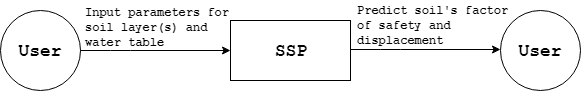
\includegraphics[width=0.6\textwidth]{SystemContextFigure.png}
		\caption{System Context}
		\label{Fig_SystemContext} 
	\end{center}
\end{figure}

The interaction between the product and the user is through a user
interface.  The responsibilities of the user and the system are as follows:

\begin{itemize}
\item User Responsibilities:
  \begin{itemize}
  \item Provide the input data related to the soil layer(s) and water table (if applicable),
    ensuring no errors in the data entry
  \item Ensure that consistent units are used for input variables
  \item Ensure required software assumptions (Section~\ref{Assumptions}) are
    appropriate for any particular problem input to the software
  \end{itemize}
\item \progname\ Responsibilities:
  \begin{itemize}
  \item Detect data type mismatch, such as a string of characters input instead
    of a floating point number
  \item Determine if the inputs satisfy the required physical
    constraints
  \item Identify the most likely failure surface within the possible input range
  \item Find the factor of safety for the slope
  \item Find the displacement of soil that will occur on the slope
  \end{itemize}
\end{itemize}

\subsection{User Characteristics}
\label{Sec:UserChar}
The end user of \progname\ should have an understanding of undergraduate
Level 1 Calculus and Physics, and be familiar with soil and material
properties.

\subsection{System Constraints}

There are no system constraints.

\section{Specific System Description}

This section first presents the problem description, which gives a
high-level view of the problem to be solved.  This is followed by the
solution characteristics specification, which presents the
assumptions, theories, definitions and finally the instance models
that model the slope. \\

\subsection{Problem Description} \label{Sec_pd}

\progname\ is a computer program developed to evaluate the factor of safety
of a slope's slip surface and, calculate the displacement the slope
will experience.

\subsubsection{Terminology}

\begin{itemize}
\item {\textit{Factor of safety:} The global stability of a surface in a slope.}
  
\item {\textit{Critical slip surface:} Slip surface of the slope that
  has the lowest global factor of safety, and therefore most likely to
  experience failure.}

\item {\textit{Stress:} Forces that are exerted between planes
  internal to a larger body subject to external loading.}
  
\item {\textit{Strain:} Stress forces that result in deformation of
  the body/plane.}
  
\item {\textit{Normal Force:} A force applied perpendicular to the
  plane of the material.}
  
\item {\textit{Shear Force:} A force applied parallel to the plane of
  the material.}
  
\item {\textit{Tension:} A stress the causes displacement of the body
  away from its center.}
  
\item {\textit{Compression:} A stress the causes displacement of the
  body towards its center.}
  
\item {\textit{Plane Strain:} The resultant stresses in one of the
  directions of a 3 dimensional material can be approximated as
  0. Results when the length of one dimension of the body dominates
  the others. Stresses in the dominant dimensions direction are the
  ones that can be approximated as 0.}
  
\end{itemize}

\subsubsection{Physical System Description} \label{sec_system}

Analysis of the slope is performed by looking at properties of the
slope as a series of slice elements. Some properties are interslice
properties, and some are slice or slice base properties.  The index
convention for referencing which interslice or slice is being used is
shown in \fref{Fig_Index}.

\begin{itemize}
\item Interslice properties convention is noted by $\text{j}$. The end
  Interslice properties are usually not of interest, therefore use the
  interslice properties from $1\leq\text{i}\leq n-1$.

\item Slice properties convention is noted by $\text{i}$.
\end{itemize}


\begin{figure}[h!] \refstepcounter{fnum}  \label{Fig_Index}
\begin{center}
{
\setlength{\unitlength}{6cm}
\begin{picture}(2,1)
% BORDER %
\thinlines
\put(0,0){\line(0,1){1}}
\put(0,1){\line(1,0){2}}
\put(2,1){\line(0,-1){1}}
\put(2,0){\line(-1,0){2}}
% SLIP SURFACE %
\linethickness{1mm}
\qbezier(0.2, 0.9)(0.5, 0.3)(1.8, 0.1)
% SLOPE %
\linethickness{0.1mm}
\put(0.1,0.9){\line(1,0){0.5}}
\put(0.6,0.9){\line(3,-2){1.2}}
\put(1.8,0.1){\line(1,0){0.1}}
% SLICES %
\put(0.2,0.9){\line(0,1){0}}
\put(0.6,0.484){\line(0,1){0.416}}
\put(0.992,0.2938){\line(0,1){0.3401}}
\put(1.4005,0.1764){\line(0,1){0.19}}
\put(1.8,0.1){\line(0,1){0}}
% j LABELS %
\put(0.15,0.92){$j=0$}
\put(0.55,0.92){$j=1$}
\put(1.3985,0.3863){$j=n-1$}
\put(1.78,0.13){$j=n$}
% j LABELS %
\put(0.38,0.75){$i=1$}
\put(0.74,0.55){$i=2$}
\put(1.1,0.34){$i=n-1$}
\put(1.48,0.185){$i=n$}
\end{picture}
}
\caption{Index convention for numbering slice and interslice force
  variables}
 \end{center}
\end{figure}


~\newline\noindent A free body diagram of the forces acting on the
slice is displayed in \fref{Fig_Forces}.

\begin{figure}[h!] \refstepcounter{fnum}  \label{Fig_Forces}
\begin{center}
{
 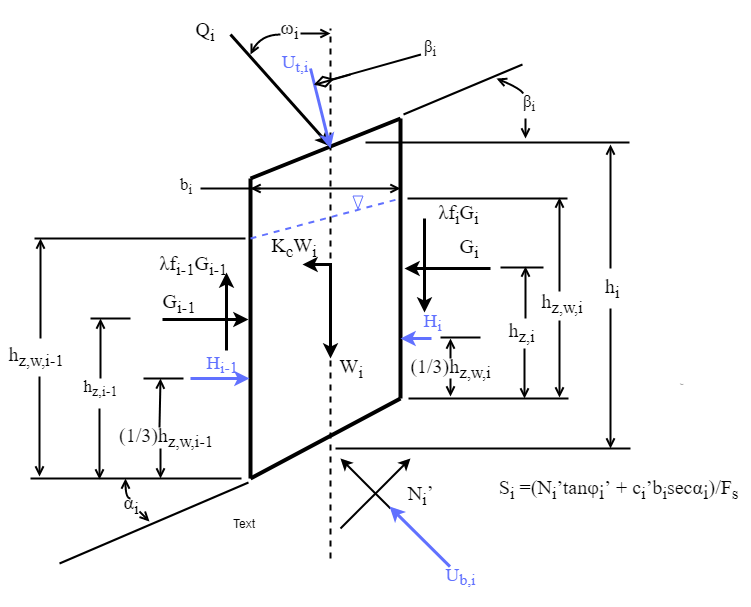
\includegraphics[width=0.7\textwidth]{ForceDiagram.png}
}
\caption{Forces acting on a slice (Note: Instances of $E$ in the figure is to be relabelled $G$)}
\end{center}
\end{figure}



\subsubsection{Goal statements}

Given the geometry of the water table, the geometry of the layers
composing the plane of a slope, and the material properties of the
layers, the goal statements are:

\begin{itemize}
\item [G\refstepcounter{goalnum}\thegoalnum: \label{G_FS}]
  {Evaluate local and global factors of safety along a given slip
    surface.}
  
\item [G\refstepcounter{goalnum}\thegoalnum: \label{G_Critical}]
  {Identify the critical slip surface for the slope, with the lowest
    factor of safety.}
  
\item [G\refstepcounter{goalnum}\thegoalnum: \label{G_Displacement}]
  {Determine the displacement of the slope.}
\end{itemize}

\subsection{Solution Characteristics Specification}

The instance models that govern \progname\ are presented in
Section~\ref{sec_instance}.  The information to understand the
meaning of the instance models and their derivation is also presented,
so that the instance models can be verified.

\subsubsection{Assumptions}
\label{Assumptions}
This section simplifies the original problem and helps in developing
the theoretical model by filling in the missing information for the
physical system.
The numbers given in the square brackets refer to the data definition, or the instance model, in which the respective
 assumption is used.

\begin{enumerate}[label=A\arabic*:,ref={\arabic*}]
\item [A\refstepcounter{assumpnum}\theassumpnum: \label{A_Concave}] The
  slip surface is concave with respect to the slope surface. The (x,y)
  coordinates of the failure surface follow a monotonic function.

\item [A\refstepcounter{assumpnum}\theassumpnum: \label{A_Input}] The
  geometry of the slope, and the material properties of the soil
  layers are given as inputs. [\iref{IM_RFEM}]

\item [A\refstepcounter{assumpnum}\theassumpnum: \label{A_Homo}] The
  different layers of the soil are homogeneous, with consistent soil
  properties throughout, and independent of dry or saturated
  conditions, with the exception of unit weight.

\item [A\refstepcounter{assumpnum}\theassumpnum: \label{A_Isotropic}]
  Soil layers are treated as if they have isotropic properties.
  
\item [A\refstepcounter{assumpnum}\theassumpnum: \label{A_Base}]
  Interslice normal and shear forces have a linear relationship,
  proportional to a constant $\left({\lambda}\right)$ and an
  interslice force function $\left({f}\right)$ depending on x
  position.

\item [A\refstepcounter{assumpnum}\theassumpnum: \label{A_Interslice}]
  Slice to base normal and shear forces have a linear relationship,
  dependent on the factor of safety $\left({FS}\right)$, and the
  Coulomb sliding law.

\item
  [A\refstepcounter{assumpnum}\theassumpnum: \label{A_StressStrain}]
  The stress-strain curve for interslice relationships is linear with
  a constant slope.
  
\item [A\refstepcounter{assumpnum}\theassumpnum: \label{A_2D}] The
  slope and slip surface extends far into and out of the geometry ($z$
  coordinate). This implies plane strain conditions, making 2D
  analysis appropriate.

\item [A\refstepcounter{assumpnum}\theassumpnum: \label{A_Lin}] The
  effective normal stress is large enough that the resistive shear to
  effective normal stress relationship can be approximated as a linear
  relationship.

\item [A\refstepcounter{assumpnum}\theassumpnum: \label{A_Straight}]
  The surface and base of a slice between interslice nodes are
  approximated as straight lines.
\end{enumerate}

\subsubsection{Theoretical Models} \label{sec_theoretical}

This section focuses on the general equations and laws that \progname\ is based
on.

~\newline

% ----------------------------- %
%        Begin TM FS           %
% ----------------------------- %
\noindent
\begin{minipage}{\textwidth}
\renewcommand*{\arraystretch}{1.5}
\begin{tabular}{| p{1.5cm} | p{14cm}|}
  
  \hline Number&
  T\refstepcounter{theorynum}\thetheorynum \label{TM_FS}\\
  
  \hline Label&\bf Factor of Safety\\
  
  \hline Equation& \( \text{FS} = \frac{P}{S} \) \\
  
  \hline Description & The stability metric of the slope, known as the
  factor of safety $\text{FS}$, is determined by the ratio of the
  shear force at the base of the slope $S$, and
  the resistive shear $P$. \\
 
  \hline Source & \cite{FredlundKrahn}\\

  \hline Ref.\ By & \iref{IM_FS}, \dref{GD_MobShear} \\

  \hline
\end{tabular}
\end{minipage}\\
% ----------------------------- %
%        End TM FS              %
% ----------------------------- %

~\newline

% ----------------------------- %
%        Begin TM Equilibrium            %
% ----------------------------- %
\noindent
\begin{minipage}{\textwidth}
\renewcommand*{\arraystretch}{1.5}
\begin{tabular}{| p{1.5cm} | p{14cm}|}
  
  \hline Number&
  T\refstepcounter{theorynum}\thetheorynum \label{TM_Eqm}\\
  
  \hline
  Label&\bf Equilibrium\\
  
  \hline Equation& \( \displaystyle\sum {F}_{\text{x}} = 
  \displaystyle\sum F_{\text{y}} = \displaystyle\sum M = 0
  \)\\

  \hline Description & For a body in static equilibrium the net
  forces and net moments acting on the body will cancel out. Assuming
  a 2D problem (\aref{A_2D}) the x-component of the net force ${F_{x}}$ 
and y-component of the net force ${F_{y}}$ will be equal to $0$. All forces
 and their distance from the chosen point of rotation will create a net
 moment equal to $0$. \\
  
  \hline Source & \cite{FredlundKrahn}\\
  
  \hline Ref.\ By & \dref{GD_Fx}, \dref{GD_Fy}, \dref{GD_M},
  \iref{IM_Lambda} \\
  
  \hline
\end{tabular}
\end{minipage}\\
% ----------------------------- %
%        End TM Equilibrium   %
% ----------------------------- %

~\newline

% ----------------------------- %
%        Begin TM Mohr Coulomb            %
% ----------------------------- %
\noindent
\begin{minipage}{\textwidth}
\renewcommand*{\arraystretch}{1.5}
\begin{tabular}{| p{1.5cm} | p{14cm}|}
  
  \hline  Number&
  T\refstepcounter{theorynum}\thetheorynum \label{TM_Fmc}\\
  
  \hline Label&\bf Mohr-Coulomb Shear Strength\\
  
  \hline Equation& \( P = \sigma \cdot \tan\left( \varphi' \right) + c'
  \) \\
  
  \hline Description & For a soil under stress it will exert a shear
  resistive strength based on the Coulomb sliding law.  The resistive
  shear is the maximum amount of shear a surface can experience while
  remaining rigid, analogous to a maximum normal force.  In this model
  the shear force $P$ is proportional to the product of the normal
  stress on the plane $\sigma$ with it's static friction, in the
  angular form $\tan\left( \varphi' \right)=U_{\text{s}}$.  The $P$
  versus $\sigma$ relationship is not truly linear, but assuming the
  effective normal force is strong enough, it can be approximated with
  a linear fit (\aref{A_Lin}), where the cohesion $c'$ represents the
  $P$ intercept of the fitted line.\\

  \hline Source & \cite{FredlundKrahn}\\
  
  \hline Ref.\ By & \dref{GD_P}, \dref{GD_MobShear}, \ddref{DD_R},
  \ddref{DD_T}, \iref{IM_RFEMFS}\\
  
  \hline
\end{tabular}
\end{minipage}\\
% ----------------------------- %
%        End TM Mohr Coulomb              %
% ----------------------------- %

~\newline

% ----------------------------- %
%        Begin TM Effective Stress            %
% ----------------------------- %
\noindent
\begin{minipage}{\textwidth}
\renewcommand*{\arraystretch}{1.5}
\begin{tabular}{| p{1.5cm} | p{14cm}|}
  
  \hline  Number&
  T\refstepcounter{theorynum}\thetheorynum \label{TM_EffStress}\\
  
  \hline Label&\bf Effective Stress\\
  
  \hline Equation& \( \sigma' =\sigma - \mu \) \\
  
  \hline Description & $\sigma$ is the total stress a soil mass needs
  to maintain itself as a rigid collection of particles. The source of
  the stress can be provided by the soil skeleton $\sigma'$, or by the
  pore pressure from water within the soil $\mu$. The stress from the
  soil skeleton is known as the effective stress $\sigma'$ and is the
  difference between the total stress $\sigma$ and the pore stress
  $\mu$. \\

  \hline Source & \cite{FredlundKrahn}\\
  
  \hline Ref.\ By & \dref{GD_P}, \dref{GD_MobShear}, \ddref{DD_R},
  \ddref{DD_T}, \iref{IM_E}\\
  
  \hline
\end{tabular}
\end{minipage}
% ----------------------------- %
%        End TM Effective Stress             %
% ----------------------------- %

~\newline

% ----------------------------- %
%      Begin TM Hookes         %
% ----------------------------- %
\noindent
\begin{minipage}{\textwidth}
\renewcommand*{\arraystretch}{1.5}
\begin{tabular}{| p{1.5cm} | p{14cm}|}
  
  \hline Number&
  T\refstepcounter{theorynum}\thetheorynum \label{TM_Hooke}\\
  
  \hline Label&\bf Hooke's Law\\
  
  \hline Equation& \( {F}= {K} \cdot {\delta} \) \\
  
  \hline Description & Stiffness $K$ is the resistance of a body to deformation by displacement $\delta{}$ when subject to a force $F$, along the 
same direction. A body with high stiffness will experience little deformation when 
subject to a force. \\

  \hline Source & \cite{StolleGuo}\\

  \hline Ref.\ By & \dref{GD_NetForce}, \dref{GD_Hookes},
  \ddref{DD_Stiff}, \iref{IM_RFEM}, \iref{IM_RFEMFS}\\
  
  \hline
\end{tabular}
\end{minipage}\\


% ----------------------------- %
%        End TM Hookes         %
% ----------------------------- %

\subsubsection{General Definitions} \label{sec_gendef}

This section collects the laws and equations that will be used in
deriving the data definitions, which in turn are used to build the
instance models.

~\newline

% ------------------------------------------ %
%        Begin GD Force Equilibrium X     %
% ------------------------------------------ %
\noindent
\begin{minipage}{\textwidth}
\renewcommand*{\arraystretch}{1.5}
\begin{tabular}{| p{1.5cm} | p{14cm}|}
  
  \hline  Number&
  GD\refstepcounter{defnum}\thedefnum \label{GD_Fx}\\
  
  \hline Label&\bf Normal Force Equilibrium\\
  
  \hline Equation& \( N_{\text{i}} \; = \begin{array}{l} \left[
      W_{\text{i}} - X_{\text{i-1}} + X_{\text{i}} +
      {U_{\text{t,i}}}\;{\cos\left(\beta_{\text{i}}\right)} +
      Q_{\text{i}}\;{\cos\left(\omega_{\text{i}}\right)}
      \right]\cos\left(\alpha_{\text{i}}\right) \\ + \left[
      {-K_{\text{c}}}\;{W_{\text{i}}} - G_{\text{i}} + G_{\text{i-1}}
      - H_{\text{i}} + H_{\text{i-1}} +
      {U_{\text{t,i}}}\;{\sin\left(\beta_{\text{i}}\right)} +
      Q_{\text{i}}\;{\sin\left(\omega_{\text{i}}\right)}
      \right]\sin\left(\alpha_{\text{i}}\right) \end{array} \) \\
 
  \hline Description & For a slice of mass in the slope the force
  equilibrium to satisfy \tref{TM_Eqm} in the direction perpendicular
  to the base surface of the slice. Rearranged to solve for the normal
  force of the surface $N$. Force equilibrium is derived
  from the free body diagram of \fref {Fig_Forces} in
  section~\ref{sec_system}. Index $\text{i}$ refers to the values of
  the properties for slice/interslices following convention in
  \fref {Fig_Index} in section~\ref{sec_system}. Force variable
  definitions can be found in \ddref{DD_W} to \ddref{DD_EX}.  \\

  \hline Source & \cite{ZhuEtAl2005}\\
  
  \hline Ref.\ By & \ddref{DD_R}, \ddref{DD_T}, \iref{IM_E}\\
  
  \hline
\end{tabular}
\end{minipage}\\
% ------------------------------------------ %
%        End  GD Force Equilibrium X       %
% ------------------------------------------ %

~\newline

% ------------------------------------------ %
%        Begin GD Force Equilibrium Y     %
% ------------------------------------------ %
\noindent
\begin{minipage}{\textwidth}
\renewcommand*{\arraystretch}{1.5}
\begin{tabular}{| p{1.5cm} | p{14cm}|}
  
  \hline  Number&
  GD\refstepcounter{defnum}\thedefnum \label{GD_Fy}\\
  
  \hline Label&\bf Base Shear Force Equilibrium\\
  
  \hline Equation& \( S_{\text{i}} = \begin{array}{l} \left[
      W_{\text{i}} -X_{\text{i-1}} + X_{\text{i}} +
      {U_{\text{t,i}}}\;{\cos\left(\beta_{\text{i}}\right)} +
      Q_{\text{i}}\;{\cos\left(\omega_{\text{i}}\right)}
      \right]\sin\left(\alpha_{\text{i}}\right) \\ - \left[
      {-K_{\text{c}}}\;{W_{\text{i}}} - G_{\text{i}} + G_{\text{i-1}}
      - H_{\text{i}} + H_{\text{i-1}} +
      {U_{\text{t,i}}}\;{\sin\left(\beta_{\text{i}}\right)} +
      Q_{\text{i}}\;{\cos\left(\omega_{\text{i}}\right)}
      \right]\cos\left(\alpha_{\text{i}}\right) \end{array} \) \\
  
  \hline Description & For a slice of mass in the slope the force
  equilibrium to satisfy \tref{TM_Eqm} in the direction parallel to
  the base surface of the slice. Rearranged to solve for the shear
  force acting on the base $S_{\text{i}}$. Force equilibrium is
  derived from the free body diagram of \fref{Fig_Forces} in
  section~\ref{sec_system}. Index $\text{i}$ refers to the values of
  the properties for slice/interslices following convention in
  \fref{Fig_Index} in section~\ref{sec_system}. Force variable
  definitions can be found in \ddref{DD_W} to \ddref{DD_EX}.  \\

  \hline Source & \cite{ZhuEtAl2005}\\
  
  \hline Ref.\ By & \ddref{DD_R}, \ddref{DD_T},\iref{IM_E}\\
  
  \hline
\end{tabular}
\end{minipage}\\
% ------------------------------------------ %
%        End  GD Force Equilibrium Y       %
% ------------------------------------------ %

~\newline

% ----------------------------- %
%        Begin GD Resistive Shear   %
% ----------------------------- %
\noindent
\begin{minipage}{\textwidth}
\renewcommand*{\arraystretch}{1.5}
\begin{tabular}{| p{1.5cm} | p{14cm}|}
  
  \hline  Number&
  GD\refstepcounter{defnum}\thedefnum \label{GD_P}\\
  
  \hline Label&\bf Resistive Shear Force\\
  
  \hline Equation& \( P_{\text{i}} = N'_{\text{i}} \cdot \tan\left(
  \varphi'_{\text{i}} \right) + c' \cdot b_{\text{i}} \cdot
  \sec\left(\alpha_{\text{i}}\right) \) \\
  
  \hline Description & 
 The Mohr-Coulomb resistive shear strength of a slice $\tau{}$ from \tref{TM_Fmc} is multiplied by the area $b\sec\left(\alpha{}\right)\cdot{}1$ to obtain the resistive shear force $P$. Note the extra $1$ is to represent a unit of width which is multiplied by the total base length of a slice ${\ell{}_{b}}$ of the plane where the normal occurs, where ${\ell{}_{b}}=b\sec\left(\alpha{}\right)$ and $b$ is the x width of the base. This accounts for the effective normal force $N'=N-{U_{b}}$ of a soil from \tref{TM_EffStress} where the normal stress is multiplied by the same area to obtain the effective normal force $\sigma{}b\sec\left(\alpha{}\right)\cdot{}1=N'$.\\

  \hline Source & \cite{ZhuEtAl2005}\\
  
  \hline Ref.\ By & \dref{GD_MobShear}, \ddref{DD_R}, \ddref{DD_T}\\
  
  \hline
\end{tabular}
\end{minipage}\\
% ----------------------------- %
%        End GD Resistive Shear             %
% ----------------------------- %

~\newline

% ----------------------------- %
%  Begin GD Mobile Shear   %
% ----------------------------- %
\noindent
\begin{minipage}{\textwidth}
\renewcommand*{\arraystretch}{1.5}
\begin{tabular}{| p{1.5cm} | p{14cm}|}
  
  \hline \ Number&
  GD\refstepcounter{defnum}\thedefnum \label{GD_MobShear}\\
  
  \hline Label&\bf Mobile Shear \\
  
  \hline Equation & \( S_{\text{i}} = \frac{ P_{\text{i}} }{ \text{FS}
  } = \frac { N'_{\text{i}} \cdot \tan\left( \varphi'_{\text{i}}
    \right) + c' \cdot b_{\text{i}} \cdot
    \sec\left(\alpha_{\text{i}}\right) }{\text{FS}} \) \\
  
  \hline Description & From the definition of the Factor of Safety in
  \tref{TM_FS}, and the new definition of $P$, a new
  relation for the net mobile shear force of the slice $T$
  is found as the resistive shear $P$ (\dref{GD_P}) divided
  by the factor of safety $\text{FS}$. \\

  \hline Source & \cite{ZhuEtAl2005}\\
  
  \hline Ref.\ By & \ddref{DD_R}, \ddref{DD_T} \\
  
  \hline
\end{tabular}
\end{minipage}\\
% ----------------------------- %
%        End GD Mobile Shear             %
% ----------------------------- %

~\newline

% ------------------------------------------ %
%        Begin GD  Interslice Normal/Shear Relationship    %
% ------------------------------------------ %
\noindent
\begin{minipage}{\textwidth}
\renewcommand*{\arraystretch}{1.5}
\begin{tabular}{| p{1.5cm} | p{14cm}|}
  
  \hline  Number&
  GD\refstepcounter{defnum}\thedefnum \label{GD_X}\\
  
  \hline Label&\bf Interslice Normal/Shear Relationship\\
  
  \hline Equation& \( X = \lambda \cdot f \cdot
  G \) \\

  \hline Description & The assumption for the Morgenstern Price method
  (\aref{A_Base}) that the interslice shear force $X$ is
  proportional to the interslice normal force $G$ by a
  proportionality constant $\lambda$, and a predetermined scaling
  function $f$, that changes the proportionality as a function of the
  $x$-ordinate position of the interslice. $f$ is typically either a
  half-sine along the slip surface, or a constant.  \\

  \hline Source & \cite{ZhuEtAl2005}\\
  
  \hline Ref.\ By & \ddref{DD_R}, \ddref{DD_T}, \iref{IM_FS},
  \iref{IM_Lambda}, \iref{IM_E}\\
  
  \hline
\end{tabular}
\end{minipage}\\
% ------------------------------------------ %
%        End  GD Interslice Normal/Shear Relationship       %
% ------------------------------------------ %

~\newline

% ------------------------------------------ %
%        Begin GD Moment Equilibrium    %
% ------------------------------------------ %
\noindent
\begin{minipage}{\textwidth}
\renewcommand*{\arraystretch}{1.5}
\begin{tabular}{| p{1.5cm} | p{14cm}|}
  
  \hline  Number&
  GD\refstepcounter{defnum}\thedefnum \label{GD_M}\\
  
  \hline Label&\bf Moment Equilibrium\\
  
  \hline Equation& \( 0 = \begin{array}{l} - {G}_{\text{i}} \left[
      {z_{\text{i}}} + \frac{b_{\text{i}}}{2} {
        \tan\left(\alpha_{\text{i}}\right)} \right] + {G}_{\text{i-1}}
    \left[ {z_{\text{i-1}}} - \frac{b_{\text{i}}}{2} {
        \tan\left(\alpha_{\text{i}}\right)} \right] -
    H_{\text{i}}\left[ z_{\text{w,i}} + \frac{b_{\text{i}}}{2} {
        \tan\left(\alpha_{\text{i}}\right)} \right] \\[5pt] +
    H_{\text{i-1}}\left[ z_{\text{w,i-1}} - \frac{b_{\text{i}}}{2} {
        \tan\left(\alpha_{\text{i}}\right)} \right] +
    \frac{b_{\text{i}}}{2} \left( X_{\text{i}} + X_{\text{i-1}}
    \right) - K_{\text{c}} W_{\text{i}} \frac{h_{\text{i}}}{2} +
    U_{\text{t,i}} \sin\left(\beta_{\text{i}}\right) h_{\text{i}} \\ +
    Q_{\text{i}}\;{\sin\left(\omega_{\text{i}}\right)}
    h_{\text{i}} \end{array} \) \\

  \hline Description & For a slice of mass in the slope the moment
  equilibrium to satisfy \tref{TM_Eqm} in the direction perpendicular
  to the base surface of the slice. Moment equilibrium is derived from
  the free body diagram of \fref{Fig_Forces} in
  section~\ref{sec_system}. Index $\text{i}$ refers to the values of
  the properties for slice/interslices following convention in
  \fref{Fig_Index} in section~\ref{sec_system}.  Variable
  definitions can be found in \ddref{DD_W} to \ddref{DD_EX}.  \\

  \hline Source & \cite{ZhuEtAl2005}\\
  
  \hline Ref.\ By & \iref{IM_Lambda}\\
  
  \hline
\end{tabular}
\end{minipage}\\
% ------------------------------------------ %
%        End  GD Moment Equilibrium       %
% ------------------------------------------ %

~\newline

% ------------------------------------------ %
%        Begin GD Net X-Force      %
% ------------------------------------------ %
\noindent
\begin{minipage}{\textwidth}
\renewcommand*{\arraystretch}{1.5}
\begin{tabular}{| p{1.5cm} | p{14cm}|}
  
  \hline  Number&
  GD\refstepcounter{defnum}\thedefnum \label{GD_NetForce}\\
  
  \hline Label&\bf Net X-Component Force\\
  
  \hline Equation & \(F_{\text{x,i}} = -\Delta H_\text{i} -K_{\text{c}}
  \cdot W_\text{i} - U_{\text{b,i}} \sin\left(\alpha_\text{i}\right) +
  U_{\text{t,i}} \sin\left(\beta\right) + Q_\text{i}
  \sin\left(\omega_\text{i}\right)\)\\


  \hline Description & \\

  \hline Source & \\
  
  \hline Ref.\ By & \\
  
  \hline
\end{tabular}
\end{minipage}\\

~\newline

% ------------------------------------------ %
%        Begin GD Net Force      %
% ------------------------------------------ %
\noindent
\begin{minipage}{\textwidth}
\renewcommand*{\arraystretch}{1.5}
\begin{tabular}{| p{1.5cm} | p{14cm}|}
  
  \hline  Number&
  GD\refstepcounter{defnum}\thedefnum \label{GD_NetForce}\\
  
  \hline Label&\bf Net Y-Component Force\\
  
  \hline Equation &\(F_{\text{y,i}} = -W_\text{i} + U_{\text{b,i}}
  \cos\left(\alpha_\text{i}\right) - U_{\text{t,i}}
  \cos\left(\beta_\text{i}\right) - Q_\text{i}
  \cos\left(\omega_\text{i}\right) \)\\

  \hline Description & These equations show the net sum of the forces acting on a slice for the RFEM model and the forces that create an applied load on the slice. ${F_{x}}$ refers to the load in the direction perpendicular to the direction of the force of gravity for slice $i$, while ${F_{y}}$ refers to the load in the direction parallel to the force of gravity for slice $i$. Forces are found in the free body diagram of \fref{Fig_Forces} in section~\ref{sec_system}. In
  this model the elements are not exerting forces on each other, so
  the interslice forces $G$ and $X$ are not a part of the model. Index
  $\text{i}$ refers to the values of the properties for
  slice/interslices following convention in \fref{Fig_Index} in
  section~\ref{sec_system}. Force variable definitions can be found in
  \ddref{DD_W} to \ddref{DD_Q}.\\

  \hline Source & \cite{ZhuEtAl2005}\\
  
  \hline Ref.\ By & \ddref{DD_Eqm},
  \iref{IM_RFEM}\\
  
  \hline
\end{tabular}
\end{minipage}\\

% ------------------------------------------ %
%        End  GD Net Force       %
% ------------------------------------------ %

~\newline

% ------------------------------------------ %
%        Begin GD Hookes      %
% ------------------------------------------ %
\noindent
\begin{minipage}{\textwidth}
\renewcommand*{\arraystretch}{1.5}
\begin{tabular}{| p{3cm} | p{12.5cm}|}
  
  \hline  Number&
  GD\refstepcounter{defnum}\thedefnum \label{GD_Hookes}\\
  
  \hline Label&\bf Hooke's Law 2D\\
  
  \hline Equation&

  \( \left[\begin{array}{l} p_\text{t,i} \\ p_\text{n,i} \end{array}
    \right] = \left[ \begin{array}{l l} K_\text{t,i} & 0 \\ 0 &
      K_\text{n,i}\end{array} \right] \left[\begin{array}{l} \delta
      t_\text{i} \\ \delta n_\text{i}
    \end{array} \right] \) \\

  \hline Description & A 2D component implementation of Hooke's law as
  seen in \tref{TM_Hooke}. $\delta n_\text{i}$ is the displacement of
  the element normal to the surface and $\delta t_\text{i}$ is the
  displacement of the element parallel to the surface. $p_\text{n,i}$,
  is the net pressure acting normal to the surface, and $p_\text{t,i}$
  is the net pressure acting parallel to the surface. Pressure is used
  in place of force as the surface has not been normalized for it's
  length. The stiffness values $K_\text{n,i}$ and $K_\text{t,i}$ are
  then the resistance to displacement in the respective directions
  defined as in \ddref{DD_Stiff}. The pressure forces would be the
  result of applied loads on the mass, the product of the stiffness
  elements with the displacement would be the mass's reactive force
  that creates equilibrium with the applied forces after reaching the
  equilibrium displacement. \\

  \hline Source & \cite{StolleGuo}\\
  
  \hline Ref.\ By & \ddref{DD_KMats},
  \iref{IM_RFEM}\\
  
  \hline
\end{tabular}
\end{minipage}\\

% ------------------------------------------ %
%        End  GD Hookes       %
% ------------------------------------------ %

~\newline

% ------------------------------------------ %
%        Begin GD Displacement Vectors      %
% ------------------------------------------ %
\noindent
\begin{minipage}{\textwidth}
\renewcommand*{\arraystretch}{1.5}
\begin{tabular}{| p{3cm} | p{12.5cm}|}
  
  \hline  Number&
  GD\refstepcounter{defnum}\thedefnum \label{GD_DispVecs}\\
  
  \hline Label&\bf Displacement Vectors\\
  
  \hline Equation&

 $\varepsilon{}_{i}=\begin{bmatrix}
{\delta{}u}_{i}\\
{\delta{}v}_{i}
\end{bmatrix}=\begin{bmatrix}
\cos\left(\alpha{}_{i}\right) & \sin\left(\alpha{}_{i}\right)\\
\left(-\sin\left(\alpha{}_{i}\right)\right) & \cos\left(\alpha{}_{i}\right)
\end{bmatrix}\delta{}_{i}=\begin{bmatrix}
\cos\left(\alpha{}_{i}\right) & \sin\left(\alpha{}_{i}\right)\\
\left(-\sin\left(\alpha{}_{i}\right)\right) & \cos\left(\alpha{}_{i}\right)
\end{bmatrix}\begin{bmatrix}
{\delta{}x}_{i}\\
{\delta{}y}_{i}
\end{bmatrix}$\\

      \hline Description &  Vectors describing the displacement of slice $i$. $\delta{}$
 is the displacement in the unrotated coordinate system, where $\delta{}x$ is the 
displacement of the slice perpendicular to the direction of gravity, and $\delta{}y$ 
is the displacement of the slice parallel to the force of gravity. $\varepsilon{}$ is 
the displacement in the rotated coordinate system, where $\delta{}u$ is the 
displacement of the slice parallel to the slice base, and $\delta{}y$ is the 
displacement of the slice perpendicular to the slice base. $\varepsilon{}$ can also 
be found by rotating $\delta{}$ clockwise by the base angle, $\alpha{}$ through 
a rotation matrix as shown.\\

  \hline Source & \cite{StolleGuo}\\
  
  \hline Ref.\ By & \ddref{DD_KMats},
  \iref{IM_RFEM}, \iref{IM_RFEMFS}\\
  
  \hline
\end{tabular}
\end{minipage}\\

% ------------------------------------------ %
%        End  GD Displacement Vectors       %
% ------------------------------------------ %

\subsubsection{Data Definition} \label{sec_datadef}

This section collects and defines all the data needed to build the
instance models. Definitions \ddref{DD_W} to \ddref{DD_Q} are the
force variables that can be solved by direct analysis of given
inputs. The interslice forces \ddref{DD_EX} are force variables that
must be written in terms of \ddref{DD_W} to \ddref{DD_Q} to solve.
~\newline

% ------------------------------------------ %
%               Begin DD W    %
% ------------------------------------------ %

\noindent
\begin{minipage}{\textwidth}
\renewcommand*{\arraystretch}{1.6}
\begin{tabular}{| p{1.5cm} | p{14cm} |}
  
\hline  Number&
DD\refstepcounter{datadefnum}\thedatadefnum \label{DD_W}\\

\hline Label& \bf Weight \\

\hline
Equation & 
 $W$ = $b_{i}\begin{cases}
\left({y_{us,i}}-{y_{slip,i}}\right){\gamma{}_{Sat}}, & {y_{wt,i}}\geq{}{y_{us,i}}\\
\left({y_{us,i}}-{y_{wt,i}}\right)\gamma{}+\left({y_{wt,i}}-{y_{slip,i}}\right){\gamma{}_{Sat}}, & {y_{us,i}}>{y_{wt,i}}>{y_{slip,i}}\\
\left({y_{us,i}}-{y_{slip,i}}\right)\gamma{}, & {y_{wt,i}}\leq{}{y_{slip,i}}
\end{cases}$
\\

\hline Description & $W$ is the weight (N)\newline$b$ is the base width of a slice (m)\newline$i$ is the index\newline${y_{us}}$ is the y ordinate (m)\newline${y_{slip}}$ is the y ordinate (m)\newline${\gamma{}_{Sat}}$ is the saturated unit weight ($\frac{\text{N}}{\text{m}^{3}}$)\newline${y_{wt}}$ is the y ordinate (m)\newline$\gamma{}$ is the dry unit weight ($\frac{\text{N}}{\text{m}^{3}}$)
\\

\hline Sources& \cite{FredlundKrahn}\\

\hline Ref.\ By & \ddref{DD_R}, \ddref{DD_T}, \iref{IM_FS},
\iref{IM_Lambda}, \iref{IM_E}\\

\hline
\end{tabular}
\end{minipage}\\

% ------------------------------------------ %
%               End DD W        %
% ------------------------------------------ %

~\newline

% ------------------------------------------ %
%               Begin DD Ub    %
% ------------------------------------------ %

\noindent
\begin{minipage}{\textwidth}
\renewcommand*{\arraystretch}{1.6}
\begin{tabular}{| p{1.5cm} | p{14cm} |}
  
\hline  Number&
DD\refstepcounter{datadefnum}\thedatadefnum \label{DD_Ub}\\

\hline Label& \bf Base Water Force \\

\hline
Equation & 
${U_{b}}$ = ${\ell{}_{b,i}}\begin{cases}
\left({y_{wt,i}}-{y_{slip,i}}\right){\gamma{}_{w}}, & {y_{wt,i}}>{y_{slip,i}}\\
0, & {y_{wt,i}}\leq{}{y_{slip,i}}
\end{cases}$
\\

\hline Description & ${U_{b}}$ is the base hydrostatic force
 (N)\newline${\ell{}_{b}}$ is the total base length of a slice (m)\newline$i$ is
 the index\newline${y_{wt}}$ is the y ordinate (m)\newline${y_{slip}}$ is the
 y ordinate (m)\newline${\gamma{}_{w}}$ is the unit weight of water
 ($\frac{\text{N}}{\text{m}^{3}}$)
\\
\hline Sources& \cite{FredlundKrahn}\\

\hline Ref.\ By & \ddref{DD_R}, \ddref{DD_T}, \iref{IM_FS},
\iref{IM_Lambda}, \iref{IM_E}\\

\hline
\end{tabular}
\end{minipage}\\

% ------------------------------------------ %
%               End DD Ub        %
% ------------------------------------------ %

~\newline

% ------------------------------------------ %
%               Begin DD Ut    %
% ------------------------------------------ %

\noindent
\begin{minipage}{\textwidth}
\renewcommand*{\arraystretch}{1.6}
\begin{tabular}{| p{1.5cm} | p{14cm} |}
  
\hline  Number&
DD\refstepcounter{datadefnum}\thedatadefnum \label{DD_Ut}\\

\hline Label& \bf Surface Hydrostatic Force \\

\hline
Equation & 
${U_{t}}$ = ${\ell{}_{s,i}}\begin{cases}
\left({y_{wt,i}}-{y_{us,i}}\right){\gamma{}_{w}}, & {y_{wt,i}}>{y_{us,i}}\\
0, & {y_{wt,i}}\leq{}{y_{us,i}}
\end{cases}$
\\ 

\hline Description & ${U_{t}}$ is the surface hydrostatic force (N)\newline${\ell{}_{s}}$ is the length of an interslice surface (m)\newline$i$ is the index\newline${y_{wt}}$ is the y ordinate (m)\newline${y_{us}}$ is the y ordinate (m)\newline${\gamma{}_{w}}$ is the unit weight of water ($\frac{\text{N}}{\text{m}^{3}}$)
\\

\hline Sources & \cite{FredlundKrahn}\\

\hline Ref.\ By & \ddref{DD_R}, \ddref{DD_T}, \iref{IM_FS},
\iref{IM_Lambda}, \iref{IM_E}\\

\hline
\end{tabular}
\end{minipage}\\

% ------------------------------------------ %
%               End DD Ut        %
% ------------------------------------------ %

~\newline

% ------------------------------------------ %
%               Begin DD H    %
% ------------------------------------------ %

\noindent
\begin{minipage}{\textwidth}
\renewcommand*{\arraystretch}{1.6}
\begin{tabular}{| p{1.5cm} | p{14cm} |}
  
\hline  Number&
DD\refstepcounter{datadefnum}\thedatadefnum \label{DD_H}\\

\hline Label& \bf Interslice Water Force \\

\hline Equation & $H$ = $\begin{cases}
\frac{\left[{y_{us,i}}-{y_{slip,i}}\right]^{2}}{2}{\gamma{}_{Sat}}+\left[{y_{wt,i}}-{y_{us,i}}\right]^{2}{\gamma{}_{Sat}}, & {y_{wt,i}}\geq{}{y_{us,i}}\\
\frac{\left[{y_{wt,i}}-{y_{slip,i}}\right]^{2}}{2}{\gamma{}_{Sat}}, & {y_{us,i}}>{y_{wt,i}}>{y_{slip,i}}\\
0, & {y_{wt,i}}\leq{}{y_{slip,i}}
\end{cases}$
\\

\hline Description & $H$ is the interslice water force (N)\newline${y_{us}}$ is the y ordinate (m)\newline$i$ is the index\newline${y_{slip}}$ is the y ordinate (m)\newline${\gamma{}_{Sat}}$ is the saturated unit weight ($\frac{\text{N}}{\text{m}^{3}}$)\newline${y_{wt}}$ is the y ordinate (m)
\\

\hline Sources & \cite{FredlundKrahn}\\

\hline Ref.\ By & \ddref{DD_R}, \ddref{DD_T}, \iref{IM_FS},
\iref{IM_Lambda}, \iref{IM_E}\\

\hline
\end{tabular}
\end{minipage}\\

% ------------------------------------------ %
%               End DD H        %
% ------------------------------------------ %

~\newline

% ------------------------------------------ %
%               Begin DD Angles   %
% ------------------------------------------ %
\noindent
\begin{minipage}{\textwidth}
\renewcommand*{\arraystretch}{1.6}
\begin{tabular}{| p{1.5cm} | p{14cm} |}
  
\hline  Number&
DD\refstepcounter{datadefnum}\thedatadefnum \label{DD_Angles_alpha}\\

\hline Label& \bf Angle\\

\hline
Equation & 
\( \alpha_\text{i} = \frac{y_\text{slip,i} -
  y_\text{slip,i-1}}{x_\text{slip,i} - x_\text{slip,i-1}} \)\\

\hline
Description & $\alpha{}$ is the angle (${}^{\circ}$)\newline${y_{slip}}$
 is the y ordinate (m)\newline$i$ is the index\newline${x_{slip}}$ is the x ordinate (m)
\\

\hline Sources& \cite{FredlundKrahn}\\

\hline Ref.\ By & \ddref{DD_R}, \ddref{DD_T}, \iref{IM_FS},
\iref{IM_Lambda}, \iref{IM_E}\\

\hline
\end{tabular}
\end{minipage}\\

\noindent
\begin{minipage}{\textwidth}
\renewcommand*{\arraystretch}{1.6}
\begin{tabular}{| p{1.5cm} | p{14cm} |}
  
\hline  Number&
DD\refstepcounter{datadefnum}\thedatadefnum \label{DD_Angles_Beta}\\

\hline Label& \bf Angle \\

\hline
Equation & 
\( \beta_\text{i} = \frac{y_\text{us,i} -
  y_\text{us,i-1}}{x_\text{us,i} - x_\text{us,i-1}} \)\\

\hline
Description & $\beta{}$ is the angle (${}^{\circ}$)\newline${y_{us}}$ is 
the y ordinate (m)\newline$i$ is the index\newline${x_{us}}$ is the x ordinate (m)
\\

\hline Sources& \cite{FredlundKrahn}\\

\hline Ref.\ By & \ddref{DD_R}, \ddref{DD_T}, \iref{IM_FS},
\iref{IM_Lambda}, \iref{IM_E}\\

\hline
\end{tabular}
\end{minipage}\\

% ------------------------------------------ %
%               End DD Angles        %
% ------------------------------------------ %

~\newline

% ------------------------------------------ %
%               Begin DD b   %
% ------------------------------------------ %

\noindent
\begin{minipage}{\textwidth}
\renewcommand*{\arraystretch}{1.6}
\begin{tabular}{| p{1.5cm} | p{14cm} |}
  
\hline  Number&
DD\refstepcounter{datadefnum}\thedatadefnum \label{DD_b}\\

\hline Label& \bf Base Width of a Slice \\

\hline
Equation & 
$b$ = ${x_{slip,i}}-{x_{slip,i-1}}$\\

\hline Description & $b$ is the base width of a slice (m)\newline${x_{slip}}$ is the x ordinate (m)\newline$i$ is the index
\\

\hline Sources& \cite{FredlundKrahn}\\

\hline Ref.\ By & \ddref{DD_R}, \ddref{DD_T}, \iref{IM_FS},
\iref{IM_Lambda}, \iref{IM_E}\\

\hline
\end{tabular}
\end{minipage}\\

\noindent
\begin{minipage}{\textwidth}
\renewcommand*{\arraystretch}{1.6}
\begin{tabular}{| p{1.5cm} | p{14cm} |}
  
\hline  Number&
DD\refstepcounter{datadefnum}\thedatadefnum \label{DD_b}\\

\hline Label& \bf Total Base Length of a Slice \\

\hline
Equation & 
${\ell{}_{b}}$ = $b_{i}\sec\left(\alpha{}_{i}\right)$\\

\hline Description & ${\ell{}_{b}}$ is the total base length of a slice (m)\newline$b$ is the base width of a slice (m)\newline$i$ is the index\newline$\alpha{}$ is the angle (${}^{\circ}$)
\\ 

\hline Sources& \cite{FredlundKrahn}\\

\hline Ref.\ By & \ddref{DD_R}, \ddref{DD_T}, \iref{IM_FS},
\iref{IM_Lambda}, \iref{IM_E}\\

\hline
\end{tabular}
\end{minipage}\\

\noindent
\begin{minipage}{\textwidth}
\renewcommand*{\arraystretch}{1.6}
\begin{tabular}{| p{1.5cm} | p{14cm} |}
  
\hline  Number&
DD\refstepcounter{datadefnum}\thedatadefnum \label{DD_b}\\

\hline Label& \bf Length of an Interslice Surface \\

\hline
Equation & 
${\ell{}_{s}}$ = $b_{i}\sec\left(\beta{}_{i}\right)$\\

\hline Description &${\ell{}_{s}}$ is the length of an interslice surface (m)\newline$b$ is the base width of a slice (m)\newline$i$ is the index\newline$\beta{}$ is the angle (${}^{\circ}$)
\\
\hline Sources& \cite{FredlundKrahn}\\

\hline Ref.\ By & \ddref{DD_R}, \ddref{DD_T}, \iref{IM_FS},
\iref{IM_Lambda}, \iref{IM_E}\\

\hline
\end{tabular}
\end{minipage}\\

% ------------------------------------------ %
%               End DD b        %
% ------------------------------------------ %

~\newline

% ------------------------------------------ %
%               Begin DD Kc  %
% ------------------------------------------ %

\noindent
\begin{minipage}{\textwidth}
\renewcommand*{\arraystretch}{1.6}
\begin{tabular}{| p{1.5cm} | p{14cm} |}
  
\hline  Number&
DD\refstepcounter{datadefnum}\thedatadefnum \label{DD_Kc}\\

\hline Label& \bf Earthquake Load Factor\\

\hline Equation & ${K_{c}}$ = ${K_{c}}W_{i}$ \\

\hline Description &${K_{c}}$ is the earthquake load factor\newline$W$ is the weight (N)\newline$i$ is the index
\\ 

\hline Sources& \cite{FredlundKrahn}\\

\hline Ref.\ By & \ddref{DD_R}, \ddref{DD_T}, \iref{IM_FS},
\iref{IM_Lambda}, \iref{IM_E}\\

\hline
\end{tabular}
\end{minipage}\\

% ------------------------------------------ %
%               End DD Kc        %
% ------------------------------------------ %

~\newline

% ------------------------------------------ %
%               Begin DD Q  %
% ------------------------------------------ %

\noindent
\begin{minipage}{\textwidth}
\renewcommand*{\arraystretch}{1.6}
\begin{tabular}{| p{1.5cm} | p{14cm} |}
  
\hline  Number&
DD\refstepcounter{datadefnum}\thedatadefnum \label{DD_Q}\\

\hline Label& \bf Imposed Surface Loads \\

\hline Equation & $Q$ = $Q_{i}\omega{}_{i}$\\

\hline Description & $Q$ is the imposed surface load (N)\newline$i$ is the index\newline$\omega{}$ is the angle (${}^{\circ}$)  \\

\hline Sources& \cite{ZhuEtAl2005}\\

\hline Ref.\ By & \ddref{DD_R}, \ddref{DD_T}, \iref{IM_FS},
\iref{IM_Lambda}, \iref{IM_E}\\

\hline
\end{tabular}
\end{minipage}\\

% ------------------------------------------ %
%               End DD Q        %
% ------------------------------------------ %

~\newline

% ------------------------------------------ %
%               Begin DD E,X  %
% ------------------------------------------ %

\noindent
\begin{minipage}{\textwidth}
\renewcommand*{\arraystretch}{1.6}
\begin{tabular}{| p{1.5cm} | p{14cm} |}
  
\hline  Number&
DD\refstepcounter{datadefnum}\thedatadefnum \label{DD_EX}\\

\hline Label& \bf Interslice ShearForces \\

\hline Equation & $X$ = $\lambda{}f_{i}G_{i}$ \\

\hline Description & $X$ is the interslice shear force (N)\newline$\lambda{}$ is the interslice normal/shear force ratio\newline$f$ is the scaling function\newline$i$ is the index\newline$G$ is the interslice normal force (N)
\\

\hline Sources& \cite{ZhuEtAl2005}\\

\hline Ref.\ By & \ddref{DD_R}, \ddref{DD_T}, \iref{IM_FS},
\iref{IM_Lambda}, \iref{IM_E}\\

\hline
\end{tabular}
\end{minipage}\\

% ------------------------------------------ %
%               End DD E,X        %
% ------------------------------------------ %

~\newline

% ------------------------------------------ %
%               Begin DD R    %
% ------------------------------------------ %

\noindent
\begin{minipage}{\textwidth}
\renewcommand*{\arraystretch}{1.6}
\begin{tabular}{| p{1.5cm} | p{14cm} |}
  
\hline  Number&
DD\refstepcounter{datadefnum}\thedatadefnum \label{DD_R}\\

\hline Label& \bf Resistive Shear, Without Interslice Forces \\

\hline
Equation & 
$R = \begin{array}{l}
  \left( \begin{array}{l}
    \left[ W_{\text{i}} + U_{\text{t,i}}
      \cos\left(\beta_{\text{i}}\right) + Q_{\text{i}}
      \cos\left(\omega_{\text{i}}\right) \right]
    \cos\left(\alpha_{\text{i}}\right) \\
+ \left[ - K_{\text{c}} W_{\text{i}} - \Delta H_{\text{i}} +
  U_{\text{t,i}} \sin\left(\beta_{\text{i}}\right) + Q_{\text{i}}
  \sin\left(\omega_{\text{i}}\right) \right]
\sin\left(\alpha_{\text{i}}\right) - U_{\text{b,i}} \end{array}
  \right) \cdot \tan\left(\varphi'\right) \\
+ c'_{\text{i}} \cdot b_{\text{i}} \cdot
\sec\left(\alpha_{\text{i}}\right) \end{array} \)\\

\hline Description & $R$ is the resistive shear force (N)\newline$W$ is the weight (N)\newline$i$ is the index\newline${U_{t}}$ is the surface hydrostatic force (N)\newline$\beta{}$ is the angle (${}^{\circ}$)\newline$Q$ is the imposed surface load (N)\newline$\omega{}$ is the angle (${}^{\circ}$)\newline$\alpha{}$ is the angle (${}^{\circ}$)\newline${K_{c}}$ is the earthquake load factor\newline$\Delta{}H$ is the difference between interslice forces (N)\newline${U_{b}}$ is the base hydrostatic force (N)\newline$\varphi{}'$ is the effective angle of friction (${}^{\circ}$)\newline$c'$ is the effective cohesion (Pa)\newline$b$ is the base width of a slice (m)
\\

\hline Sources& \cite{ZhuEtAl2005}\\

\hline Ref.\ By & \iref{IM_FS}\\

\hline
\end{tabular}
\end{minipage}\\

% ------------------------------------------ %
%               End DD R         %
% ------------------------------------------ %

\subsubsection*{Resistive Shear Force, Without the
  Influence of Interslice Forces Derivation}

\noindent
The resistive shear force of a slice is defined as $P_\text{i}$ in
\dref{GD_P}.  The effective normal in the equation for $P_\text{i}$ of
the soil is defined in the perpendicular force equilibrium of a slice
from \dref{GD_Fy}, Using the effective normal $N'_\text{i}$ of
\tref{TM_EffStress} shown in equation~(\ref{eq:N'}).

\begin{equation} \label{eq:N'}
 N'_{\text{i}} \; = \begin{array}{l}
   \left[ W_{\text{i}} - X_{\text{i-1}} + X_{\text{i}} +
     {U_{\text{t,i}}}\;{\cos\left(\beta_{\text{i}}\right)} +
     Q_{\text{i}}\;{\cos\left(\omega_{\text{i}}\right)}
     \right]\cos\left(\alpha_{\text{i}}\right) \\ + \left[
     {-K_{\text{c}}}\;{W_{\text{i}}} - G_{\text{i}} + G_{\text{i-1}} -
     H_{\text{i}} + H_{\text{i-1}} +
     {U_{\text{t,i}}}\;{\sin\left(\beta_{\text{i}}\right)} +
     Q_{\text{i}}\;{\sin\left(\omega_{\text{i}}\right)}
     \right]\sin\left(\alpha_{\text{i}}\right) \\ -
   U_{\text{b,i}} \end{array}
 \end{equation}

\noindent
The values of the interslice forces $G$ and $X$ in the equation are
unknown, while the other values are found from the physical force
definitions of \ddref{DD_W} to \ddref{DD_EX}.  Consider a force
equilibrium without the affect of interslice
forces, to obtain a solvable value as done for $N^*_\text{i}$ in
equation~(\ref{eq:N*}).

\begin{equation} \label{eq:N*}
 N^*_{\text{i}} \; = \begin{array}{l}
   \left[ W_{\text{i}} +
     {U_{\text{t,i}}}\;{\cos\left(\beta_{\text{i}}\right)} +
     Q_{\text{i}}\;{\cos\left(\omega_{\text{i}}\right)}
     \right]\cos\left(\alpha_{\text{i}}\right) \\ + \left[
     {-K_{\text{c}}}\;{W_{\text{i}}}- H_{\text{i}} + H_{\text{i-1}} +
     {U_{\text{t,i}}}\;{\sin\left(\beta_{\text{i}}\right)} +
     Q_{\text{i}}\;{\sin\left(\omega_{\text{i}}\right)}
     \right]\sin\left(\alpha_{\text{i}}\right) -
   U_{\text{b,i}} \end{array}
\end{equation}

\noindent
Using $N^*_\text{i}$, a resistive shear force neglecting the influence
of interslice forces can be solved for in terms of all known values as
done in equation~(\ref{eq:R}).

\begin{equation*}
R_\text{i} = N^*_\text{i} \tan\left(\varphi'\right) + c'_\text{i}
\cdot b'_\text{i} \sec\left(\alpha_text{i}'\right)
\end{equation*}

\begin{equation}\label{eq:R}   R_{\text{i}} \; =
  \left( \begin{array}{l} \left[ W_{\text{i}} + U_{\text{t,i}}
      \cos\left(\beta_{\text{i}}\right) + Q_{\text{i}}
      \cos\left(\omega_{\text{i}}\right) \right]
    \cos\left(\alpha_{\text{i}}\right) \\ + \left[ - K_{\text{c}}
      W_{\text{i}} - \Delta H_{\text{i}} + U_{\text{t,i}}
      \sin\left(\beta_{\text{i}}\right) + Q_{\text{i}}
      \sin\left(\omega_{\text{i}}\right) \right]
    \sin\left(\alpha_{\text{i}}\right) - U_{\text{b,i}} \end{array}
  \right) \cdot \tan\left(\varphi'\right) + c'_{\text{i}} \cdot
  b_{\text{i}} \cdot \sec\left(\alpha_{\text{i}}\right)
 \end{equation}

~\newline

% ------------------------------------------ %
%               Begin DD T    %
% ------------------------------------------ %

\noindent
\begin{minipage}{\textwidth}
\renewcommand*{\arraystretch}{1.6}
\begin{tabular}{| p{1.5cm} | p{14cm} |}
  
\hline
Number& DD\refstepcounter{datadefnum}\thedatadefnum \label{DD_T}\\

\hline
Label& \bf Mobile Shear, Without Interslice Forces \\

\hline
Equation &
$T$ = $\left(W_{i}+{U_{t,i}}\cos\left(\beta{}_{i}\right)+Q_{i}\cos\left(\omega{}_{i}\right)\right)\sin\left(\alpha{}_{i}\right)-\left(-{K_{c}}W_{i}-{\Delta{}H}_{i}+{U_{t,i}}\sin\left(\beta{}_{i}\right)+Q_{i}\sin\left(\omega{}_{i}\right)\right)\cos\left(\alpha{}_{i}\right)$
\\ 

\hline Description &  $T$ is the mobilized shear force (N)\newline$W$ is the weight (N)\newline$i$ is the index\newline${U_{t}}$ is the surface hydrostatic force (N)\newline$\beta{}$ is the angle (${}^{\circ}$)\newline$Q$ is the imposed surface load (N)\newline$\omega{}$ is the angle (${}^{\circ}$)\newline$\alpha{}$ is the angle (${}^{\circ}$)\newline${K_{c}}$ is the earthquake load factor\newline$\Delta{}H$ is the difference between interslice forces (N)
\\

\hline
Sources& \cite{ZhuEtAl2005}\\

\hline Ref.\ By & \iref{IM_FS}\\

\hline
\end{tabular}
\end{minipage}\\

% ------------------------------------------ %
%               End DD T         %
% ------------------------------------------ %

\subsubsection*{Mobile Shear Force, Without the
  Influence of Interslice Forces Derivation}

\noindent
The mobile shear force acting on a slice is defined as $S_\text{i}$
from the force equilibrium in \dref{GD_Fy},also shown in
equation~(\ref{eq:Si}).

\begin{equation}  \label{eq:Si}
  S_{\text{i}} = \begin{array}{l} \left[ W_{\text{i}} -X_{\text{i-1}}
      + X_{\text{i}} +
      {U_{\text{t,i}}}\;{\cos\left(\beta_{\text{i}}\right)} +
      Q_{\text{i}}\;{\cos\left(\omega_{\text{i}}\right)}
      \right]\sin\left(\alpha_{\text{i}}\right) \\ - \left[
      {-K_{\text{c}}}\;{W_{\text{i}}} - G_{\text{i}} + G_{\text{i-1}}
      - H_{\text{i}} + H_{\text{i-1}} +
      {U_{\text{t,i}}}\;{\sin\left(\beta_{\text{i}}\right)} +
      Q_{\text{i}}\;{\cos\left(\omega_{\text{i}}\right)}
      \right]\cos\left(\alpha_{\text{i}}\right) \end{array}
\end{equation}

\noindent
The equation is unsolvable, containing the unknown interslice normal
force $G$ and shear force $X$.  Consider a force equilibrium without
the affect of interslice forces, to obtain the mobile shear force
without the influence of interslice forces $T$, as done in
equation~(\ref{eq:T}).n

\begin{equation}  \label{eq:T} T_{\text{i}} =
  \begin{array}{l}  
\left[ W_{\text{i}} + U_{\text{t,i}} \cos\left(\beta_{\text{i}}\right)
  + Q_{\text{i}} \cos\left(\omega_{\text{i}}\right) \right]
\sin\left(\alpha_{\text{i}}\right) \\ - \left[ - K_{\text{c}}
  W_{\text{i}} - \Delta H_{\text{i}} + U_{\text{t,i}}
  \sin\left(\beta_{\text{i}}\right) + Q_{\text{i}}
  \sin\left(\omega_{\text{i}}\right) \right]
\cos\left(\alpha_{\text{i}}\right) \end{array}
\end{equation}

\noindent
The values of $R_\text{i}$ and $T_\text{i}$ are now defined completely
in terms of the known force property values of \ddref{DD_W} to
\ddref{DD_EX}.

~\newline

% ------------------------------------------ %
%               Begin DD K Mats     %
% ------------------------------------------ %

\noindent
\begin{minipage}{\textwidth}
\renewcommand*{\arraystretch}{1.6}
\begin{tabular}{| p{1.5cm} | p{14cm} |}
  
\hline  Number&
DD\refstepcounter{datadefnum}\thedatadefnum \label{DD_KMats}\\

\hline Label& \bf Force \\

\hline Equation & $p$ = $\begin{bmatrix}
{K_{st,i}} & 0\\
0 & {K_{bn,i}}
\end{bmatrix}\begin{bmatrix}
{\delta{}x}_{i}\\
{\delta{}y}_{i}
\end{bmatrix}$
\\


\hline Description & $p$ is the pressure (Pa)\newline${K_{st}}$ is the shear stiffness ($\frac{\text{Pa}}{\text{m}}$)\newline$i$ is the index\newline${K_{bn}}$ is the normal stiffness ($\frac{\text{Pa}}{\text{m}}$)\newline$\delta{}x$ is the displacement (m)\newline$\delta{}y$ is the displacement (m)
\\

\hline Sources& \cite{StolleGuo}\\

\hline Ref.\ By & \iref{IM_RFEM}\\

\hline
\end{tabular}
\end{minipage}\\


\noindent
\begin{minipage}{\textwidth}
\renewcommand*{\arraystretch}{1.6}
\begin{tabular}{| p{1.5cm} | p{14cm} |}
  
\hline  Number&
DD\refstepcounter{datadefnum}\thedatadefnum \label{DD_KMats}\\

\hline Label& \bf Force \\

\hline Equation & $p$ = $\begin{bmatrix}
{K_{bA,i}} & {K_{bB,i}}\\
{K_{bB,i}} & {K_{bA,i}}
\end{bmatrix}\begin{bmatrix}
{\delta{}x}_{i}\\
{\delta{}y}_{i}
\end{bmatrix}$
\\


\hline Description &$p$ is the pressure (Pa)\newline${K_{bA}}$ is the effective base stiffness A ($\frac{\text{Pa}}{\text{m}}$)\newline$i$ is the index\newline${K_{bB}}$ is the effective base stiffness A ($\frac{\text{Pa}}{\text{m}}$)\newline$\delta{}x$ is the displacement (m)\newline$\delta{}y$ is the displacement (m)
\\ 

\hline Sources& \cite{StolleGuo}\\

\hline Ref.\ By & \iref{IM_RFEM}\\

\hline
\end{tabular}
\end{minipage}\\

% ------------------------------------------ %
%               End DD K Mats         %
% ------------------------------------------ %

\subsubsection*{Derivation of Stiffness Matrices}
\noindent
Using the force-displacement relationship of \dref{GD_Hookes} to
define stiffness matrix ${K_\text{st}}$, as seen in
equation~(\ref{eq:Kmat}).

\begin{equation} \label{eq:Kmat}
  {K_\text{st,i}} = \left[ \begin{array}{l l}
      K_\text{st,i} & 0 \\ 0 & K_\text{bn,i}\end{array} \right]
\end{equation}

\noindent
For interslice surfaces the stiffness constants and displacements
refer to an unrotated coordinate system, ${\delta}$ of
\dref{GD_DispVecs}. The interslice elements are left in their standard
coordinate system, and therefore are described by the same equation
from \dref{GD_Hookes}. Seen as ${K}_\text{st}$ in
\ddref{DD_KMats}. $K_\text{st}$ is the shear element in the matrix,
and $K_\text{sn}$ is the normal element in the matrix, calculated as
in \ddref{DD_Stiff}.

~\newline\noindent For basal surfaces the stiffness constants and
displacements refer to a system rotated for the base angle alpha
(\ddref{DD_Angles_alpha}). To analyze the effect of force-displacement
relationships occurring on both basal and interslice surfaces of an
element $i$ they must reference the same coordinate system. The
basal stiffness matrix must be rotated counter clockwise to align with
the angle of the basal surface. The base stiffness counter clockwise
rotation is applied in equation~(\ref{eq:Krot}) to the new matrix
$\bar{K^*_\text{i}}$.


\begin{equation} \label{eq:Krot}
  \begin{aligned} \bar{K^*_\text{i}} & = 
   \left[ \begin{array}{l l} \cos\left(\alpha_\text{i}\right) & -
       \sin\left(\alpha_\text{i}\right)\\ \sin\left(\alpha_\text{i}\right)
       & \cos\left(\alpha_\text{i}\right)\end{array} \right]
   \bar{K_\text{i}}\\ {} & = \left[ \begin{array}{l l} K_\text{bt,i}
       \cos\left(\alpha_\text{i}\right) & - K_\text{bn,i}
       \sin\left(\alpha_\text{i}\right)\\ K_\text{bt,i}
       \sin\left(\alpha_\text{i}\right) & K_\text{bn,i}
       \cos\left(\alpha_\text{i}\right)\end{array}\right]
  \end{aligned} \end{equation}

\noindent
The Hooke's law force displacement relationship of \dref{GD_Hookes}
applied to the base also references a displacement vector
$\bar{\epsilon}_\text{i}$ of \dref{GD_DispVecs} rotated for the base
angle angle of the slice $\alpha_\text{i}$. The basal displacement
vector $\bar{\epsilon}_\text{i}$ is rotated clockwise to align with
the interslice displacement vector $\bar{\delta}_\text{i}$, applying
the definition of $\bar{\epsilon}_\text{i}$ in terms of
$\bar{\delta}_\text{i}$ as seen in \dref{GD_DispVecs}. Using this with
base stiffness matrix $\bar{K^*}_\text{i}$, a basal force displacement
relationship in the same coordinate system as the interslice
relationship can be derived as done in equation~(\ref{eq:pRot}).
    
\begin{equation}\label{eq:pRot} \begin{aligned}
    \left[ \begin{array}{l} p_\text{bx,i}
        \\ p_\text{by,i} \end{array}\right]
    & = \bar{K^*_\text{i}} \; \bar{\epsilon} \\
      {} & = \left[ \begin{array}{l l} K_\text{bt,i}
      \cos\left(\alpha_\text{i}\right) & - K_\text{bn,i}
      \sin\left(\alpha_\text{i}\right)\\  K_\text{bt,i}
      \sin\left(\alpha_\text{i}\right) & K_\text{bn,i}
      \cos\left(\alpha_\text{i}\right)\end{array}\right]
      \left[ \begin{array}{l l} \cos\left(\alpha_\text{i}\right)
          &\sin\left(\alpha_\text{i}\right)\\
          -\sin\left(\alpha_\text{i}\right)
          & \cos\left(\alpha_\text{i}\right)\end{array}\right]
      \left[ \begin{array}{l} \delta x_\text{i}
          \\ \delta y_\text{i} \end{array} \right] \\
      {} & = \left[ \begin{array}{l l}
          K_\text{bt,i} \cos^2\left(\alpha_\text{i}\right)+
          K_\text{bn,i} \sin^2\left(\alpha_\text{i}\right)
          & \left(K_\text{bt,i} - K_\text{bn,i}\right)
          \sin\left(\alpha_\text{i}\right)
          \cos\left(\alpha_\text{i}\right)\\
          \left(K_\text{bt,i} - K_\text{bn,i}\right)
          \sin\left(\alpha_\text{i}\right)
          \cos\left(\alpha_\text{i}\right)
          & K_\text{bt,i} \cos^2\left(\alpha_\text{i}\right)+
          K_\text{bn,i} \sin^2\left(\alpha_\text{i}\right)
        \end{array} \right]
    \left[ \begin{array}{l} \delta x_\text{i}
        \\ \delta y_\text{i}
      \end{array} \right]\end{aligned} 
      \end{equation}

\noindent
The new effective base stiffness matrix $K'_\text{i}$,as derived in
equation~(\ref{eq:Krot}) is defined in equation~(\ref{eq:K'}). This is
seen as matrix $\bar{K}_\text{b,i}$ in
\dref{DD_KMats}. $K_\text{bt,i}$ is the shear element in the matrix,
and $K_\text{bn,i}$ is the normal element in the matrix, calculated as
in \ddref{DD_Stiff}. The notation is simplified by the introduction of
the constants $K_\text{bA,i}$ and $K_\text{bB,i}$, defined in
equations~(\ref{eq:KbA}) and (\ref{eq:KbB}) respectively.

\begin{equation} \label{eq:K'}
  \begin{aligned} & \bar{ K'_\text{i}}
     = \left[ \begin{array}{l l}
          K_\text{bt,i} \cos^2\left(\alpha_\text{i}\right)+
          K_\text{bn,i} \sin^2\left(\alpha_\text{i}\right)
          & \left(K_\text{bt,i} - K_\text{bn,i}\right)
          \sin\left(\alpha_\text{i}\right)
          \cos\left(\alpha_\text{i}\right)\\
          \left(K_\text{bt,i} - K_\text{bn,i}\right)
          \sin\left(\alpha_\text{i}\right)
          \cos\left(\alpha_\text{i}\right)
          & K_\text{bt,i} \cos^2\left(\alpha_\text{i}\right)+
          K_\text{bn,i} \sin^2\left(\alpha_\text{i}\right)
      \end{array} \right] \\
    & \bar{ K'_\text{i}} = \left[ \begin{array}{l l}
        K_\text{bA,i} & K_\text{bB,i} \\
        K_\text{bB,i} & K_\text{bA,i}
      \end{array} \right] \end{aligned} \end{equation}


\begin{equation} \label{eq:KbA}
  K_\text{bA,i} = K_\text{bt,i} \cos^2\left(\alpha_\text{i}\right)+
                 K_\text{bn,i} \sin^2\left(\alpha_\text{i}\right)
\end{equation}

\begin{equation} \label{eq:KbB}
  K_\text{bB,i} = \left(K_\text{bt,i} - K_\text{bn,i}\right)
                 \sin\left(\alpha_\text{i}\right)
                 \cos\left(\alpha_\text{i}\right)
\end{equation}


\noindent
A force-displacement relationship for an element $\text{i}$ can be
written in terms of displacements occurring in the unrotated
coordinate system $\bar{\delta}_\text{i}$ of \dref{GD_DispVecs} using
the matrix $K_\text{s,i}$, and $K_\text{b,i}$ as seen in
\ddref{DD_KMats}.

~\newline

% ------------------------------------------ %
%               Begin DD Eqm     %
% ------------------------------------------ %

\noindent
\begin{minipage}{\textwidth}
\renewcommand*{\arraystretch}{1.6}
\begin{tabular}{| p{1.5cm} | p{14.25cm} |}
  
\hline  Number&
DD\refstepcounter{datadefnum}\thedatadefnum \label{DD_Eqm}\\

\hline Label& \bf Force \\

\hline Equation &
$F$ = $\left(-{\ell{}_{s,i-1}}\right){K_{sn,i-1}}\delta{}_{i-1}+\left({\ell{}_{s,i-1}}{K_{sn,i-1}}+{\ell{}_{b,i}}{K_{bn,i}}+{\ell{}_{s,i}}{K_{sn,i}}\right)\delta{}_{i}-{\ell{}_{s,i}}{K_{sn,i}}\delta{}_{i+1}$
\\

\hline Description & $F$ is the force (N)\newline${\ell{}_{s}}$ is the length of an interslice surface (m)\newline$i$ is the index\newline${K_{sn}}$ is the normal stiffness ($\frac{\text{Pa}}{\text{m}}$)\newline$\delta{}$ is the displacement (m)\newline${\ell{}_{b}}$ is the total base length of a slice (m)\newline${K_{bn}}$ is the normal stiffness ($\frac{\text{Pa}}{\text{m}}$)
\\

\hline Sources& \cite{StolleGuo}\\

\hline Ref.\ By & \iref{IM_RFEM}\\

\hline
\end{tabular}
\end{minipage}\\

% ------------------------------------------ %
%               End DD Eqm         %
% ------------------------------------------ %

~\newline

% ------------------------------------------ %
%               Begin DD Soil Stiffness     %
% ------------------------------------------ %

\noindent
\begin{minipage}{\textwidth}
\renewcommand*{\arraystretch}{1.6}
\begin{tabular}{| p{1.5cm} | p{14cm} |}
  
\hline  Number&
DD\refstepcounter{datadefnum}\thedatadefnum \label{DD_Stiff}\\

\hline Label& \bf Shear Stiffness \\

\hline Input & $G$ , $\nu$ , $b$ , $c$ , $\sigma$ , $\phi$ , $\kappa$ ,
$a$ , $A$ , $u$ , $v$\\

\hline
Output & 
${K_{bt}}$ = $\frac{G}{2\left(1+\nu{}\right)}\frac{0.1}{b}+\frac{{c'}_{i}-\sigma{}\tan\left({\varphi{}'}_{i}\right)}{|\delta{}u|+a}$
\\

\hline Description &  ${K_{bt}}$ is the shear stiffness ($\frac{\text{Pa}}{\text{m}}$)\newline$G$ is the interslice normal force (N)\newline$\nu{}$ is the Poisson's ratio\newline$b$ is the base width of a slice (m)\newline$c'$ is the effective cohesion (Pa)\newline$i$ is the index\newline$\sigma{}$ is the normal stress (Pa)\newline$\varphi{}'$ is the effective angle of friction (${}^{\circ}$)\newline$\delta{}u$ is the displacement (m)\newline$a$ is the constant (m)
\\

\hline Sources& \cite{StolleGuo}\\

\hline Ref.\ By & \iref{IM_RFEM}, \iref{IM_RFEMFS}\\

\hline
\end{tabular}
\end{minipage}\\


\noindent
\begin{minipage}{\textwidth}
\renewcommand*{\arraystretch}{1.6}
\begin{tabular}{| p{1.5cm} | p{14cm} |}
  
\hline Number&
DD\refstepcounter{datadefnum}\thedatadefnum \label{DD_Stiff}\\

\hline Label& \bf Normal Stiffness \\

\hline Input & $G$ , $\nu$ , $b$ , $c$ , $\sigma$ , $\phi$ , $\kappa$
$a$ , $A$ , $u$ , $v$\\

\hline
Output & 
${K_{bn}}$ = $\begin{cases}
\frac{G\left(1-\nu{}\right)}{\left(1+\nu{}\right)\left(1-2\nu{}+b\right)}, & \nu{}<0\\
0.01\frac{G\left(1-\nu{}\right)}{\left(1+\nu{}\right)\left(1-2\nu{}+b\right)}+\frac{\kappa{}}{\delta{}v+A}, & \nu{}\geq{}0
\end{cases}$
\\

\hline Description & ${K_{bn}}$ is the normal stiffness ($\frac{\text{Pa}}{\text{m}}$)\newline$G$ is the interslice normal force (N)\newline$\nu{}$ is the Poisson's ratio\newline$b$ is the base width of a slice (m)\newline$\kappa{}$ is the constant (Pa)\newline$\delta{}v$ is the displacement (m)\newline$A$ is the constant (m)
\\

\hline Sources& \cite{StolleGuo}\\

\hline Ref.\ By & \iref{IM_RFEM}, \iref{IM_RFEMFS}\\

\hline
\end{tabular}
\end{minipage}\\

% ------------------------------------------ %
%               End DD Soil Stiffness         %
% ------------------------------------------ %


\subsubsection{Instance Models} \label{sec_instance}

This section transforms the problem defined in the
Section~\ref{Sec_pd} into one which is expressed in mathematical
terms. It uses concrete symbols defined in Section~\ref{sec_datadef}
to replace the abstract symbols in the models identified in the
Sections~\ref{sec_theoretical} and ~\ref{sec_gendef}.

~\newline\noindent The Morgenstern Price Method is a vertical slice,
limit equilibrium slope stability analysis method. Analysis is
performed by breaking the assumed failure surface into a series of
vertical slices of mass. Static equilibrium analysis using two force
equilibrium, and one moment equation as in \tref{TM_Eqm}. The problem
is statically indeterminate with only these 3 equations and one
constitutive equation (the Mohr Coulomb shear strength of
\tref{TM_Fmc}) so the assumption of \dref{GD_X} is used. Solving for
force equilibrium allows definitions of all forces in terms of the
physical properties of \ddref{DD_W} to \ddref{DD_EX}, as done in
\ddref{DD_R}, \ddref{DD_T}.

~\newline\noindent The values of the interslice normal force $G$ the
interslice normal/shear force magnitude ratio $\lambda$, and the
Factor of Safety $\text{FS}$, are unknown. Equations for the unknowns
are written in terms of only the values in \ddref{DD_W} to
\ddref{DD_EX}, the values of $R$, and $T$ in
\ddref{DD_R} and \ddref{DD_T}, and each other. The relationships
between the unknowns are non linear, and therefore explicit equations
cannot be derived and an iterative solution method is required.


~\newline

% ------------------------------------------ %
%               Begin IM Factor of safety      %
% ------------------------------------------ %

\noindent
\begin{minipage}{\textwidth}
\renewcommand*{\arraystretch}{1.6}
\begin{tabular}{| p{1.5cm} | p{14cm} |}
  
\hline  Number&
IM\refstepcounter{instnum}\theinstnum \label{IM_FS}\\

\hline Label& \bf Factor of Safety \\

\hline Input & ${\Psi_{\text{v}}}$ , ${\Phi_{\text{v}}}$ ,
${T_{\text{v}}}$ , ${R_{\text{v}}}$ \\

\hline
Output &
\( {FS}= \frac{\displaystyle\sum_{v=1}^{n-1} \left[ {R_{v}}
    \;{\displaystyle\prod_{c=i}^{n-1} \frac{\Psi_{u}}{\Phi_{u}}
    }\right] + {R_{n}} }{\displaystyle\sum_{v=1}^{n-1} \left[ {T_{v}}
    \;{\displaystyle\prod_{c=i}^{n-1} \frac{\Psi_{u}}{\Phi_{u}}
    }\right] + {T_{n}} } \)\\

\hline Description & Equation for the Factor of Safety, the ratio
between resistive and mobile shear the slip surface. The sum of values
from each slice is taken to find the total resistive and mobile shear
for the slip surface. The constants $\Phi$ and $\Psi$ convert the
resistive and mobile shear without the influence of interslice forces,
to a calculation considering the interslice forces. \\

\hline Sources& \cite{ZhuEtAl2005}\\

\hline Ref.\ By & \iref{IM_Lambda}, \iref{IM_E}\\

\hline
\end{tabular}
\end{minipage}\\

% ------------------------------------------ %
%               End IM Factor of Safety         %
% ------------------------------------------ %

\subsubsection*{Factor of Safety Derivation}

\noindent
Using equation~(\ref{eq:Interslice2}) from
section~\ref{sec:Ederivation}, rearranging, and applying the boundary
condition that $E_{\text{0}}$ and $E_{\text{n}}$ are equal to $0$ an
equation for the factor of safety is found as equation~(\ref{eq:FS}),
also seen in \iref{IM_FS}.

\begin{equation}\label{eq:FS}
  \text{FS}= \frac{\displaystyle\sum_{v=1}^{n-1} \left[ {R_{v}}
      \;{\displaystyle\prod_{c=v}^{n-1} \frac{\Psi_{u}}{\Phi_{u}}
      }\right] + {R_{n}} }{\displaystyle\sum_{v=1}^{n-1} \left[
      {T_{v}} \;{\displaystyle\prod_{c=v}^{n-1}
        \frac{\Psi_{u}}{\Phi_{u}} }\right] + {T_{n}} }
\end{equation}

\noindent
The constants $\Psi$ and $\Phi$ described in equations \ref{eq:Psi}
and \ref{eq:Phi} are functions of the unknowns: the interslice
normal/shear force ratio $\lambda$ (\iref{IM_Lambda}) and the Factor
of Safety $\text{FS}$ (\iref{IM_FS}).

~\newline

% ------------------------------------------ %
%               Begin IM Lambda      %
% ------------------------------------------ %

\noindent
\begin{minipage}{\textwidth}
\renewcommand*{\arraystretch}{1.6}
\begin{tabular}{| p{1.5cm} | p{14cm} |}
  
\hline  Number&
IM\refstepcounter{instnum}\theinstnum \label{IM_Lambda}\\

\hline Label& \bf Normal/Shear Force Ratio \\

\hline Input & $b_{\text{v}}$ , $E_{\text{v}}$ , $H_{\text{v}}$ ,
$\alpha_{\text{v}}$ , $h_{\text{v}}$ , $W_{\text{v}}$ ,
$U_{\text{t,v}}$ , $\beta_{\text{v}}$ , $f_{\text{v}}$ ,
${K_{\text{c}}}$ \\

\hline
Output & 
\( {C1_{\text{i}}}= \) 
\(  \left\{
\renewcommand{\arraystretch}{2}
\begin{tabular}{ p{6.5cm} r} 
  $ {{b}_{\text{1}}}\left[{{E}_{\text{1}} + {H}_{\text{1}}}
    \right]{\tan\left(\alpha_{\text{1}}\right) } $ &  $
  \text{i}={\text{1}} $ \\
\noindent\parbox[c]{\hsize} {$ {{b}_{\text{i}}} \left[
    \left({{E}_{\text{i}} + {E}_{\text{i-1}}}\right) +
    \left({{H}_{\text{i}} + {H}_{\text{i-1}}}\right)
    \right]{\tan\left(\alpha_{\text{i}}\right)} \\ +
  {{h}_{\text{i}}}\left( {K_{\text{c}}}\;{W_{\text{i}}} -
  {2}\;{U_{\text{t,i}}}\;{\sin\left(\beta_{\text{i}}\right)} -
  {2}\;{Q_{\text{i}}}\;{\cos\left(\omega_{\text{i}}\right)} \right) $}
&  $ 2\leq\text{i}\leq{\text{n-1}} $ \\ $
                {{b}_{\text{n}}}\left[{{E}_{\text{n-1}} +
                    {H}_{\text{n-1}}}\right]{\tan\left(\alpha_{\text{n-1}}\right)
                } $ &  $ \text{i}=\text{n} $ \\
\end{tabular} 
\renewcommand{\arraystretch}{1}
\right. \)
~\newline~\newline
\( {C2_{\text{i}}}= \)
\(  \left\{
\renewcommand{\arraystretch}{2}
\begin{tabular}{ p{7cm} r} 
  $ {{b}_{\text{1}}}{{E}_{\text{1}}}{f_{\text{1}}} $ &  $
  \text{i}=\text{1} $ \\ $ {{b}_{\text{i}}}\;{\left({
      {f_{\text{i}}}{{E}_{\text{i}}} +
      {f_{\text{i-1}}}{{E}_{\text{i-1}}} }\right)} $ &  $
  2\leq\text{i}\leq{\text{n-1}} $ \\ $
  {{b}_{\text{n}}}{{E}_{\text{n-1}}}{f_{\text{n-1}}} $ &  $
  \text{v}=\text{n} $ \\
\end{tabular} 
\renewcommand{\arraystretch}{1}
\right. \) 
~\newline
\( \lambda= \frac{ \displaystyle\sum_{i=1}^{n} {C1_{\text{i}}}}
   {\displaystyle\sum_{i=1}^{n} {C2_{\text{i}}}} \) \\

\hline Description & $\lambda$ is the magnitude ratio between shear
and normal forces at the interslice interfaces as the assumption of
the Morgenstern Price method in \dref{GD_X}. The inclination function
$f$ determines the relative magnitude ratio between the different
interslices, while $\lambda$ determines the magnitude. $\lambda$ uses
the sum of interslice normal and shear forces taken from each
interslice. \\

\hline Sources& \cite{ZhuEtAl2005}\\

\hline Ref.\ By & \iref{IM_FS}, \iref{IM_E} \\

\hline
\end{tabular}
\end{minipage}\\

% ------------------------------------------ %
%               End IM Lambda         %
% ------------------------------------------ %

\subsubsection*{Normal/Shear Force Ratio Derivation}

 The last static equation of \tref{TM_Eqm} the moment equilibrium of
 \dref{GD_M} about the midpoint of the base is taken, with the
 assumption of \dref{GD_X}. Results in equation~(\ref{eq:Moment}).

\begin{equation}\label{eq:Moment}
  0 = \begin{array}{l} - {G}_{\text{i}} \left[ {z_{\text{i}}} -
      \frac{b_{\text{i}}}{2} { \tan\left(\alpha_{\text{i}}\right)}
      \right] + {G}_{\text{i-1}} \left[ {z_{\text{i-1}}} +
      \frac{b_{\text{i}}}{2} { \tan\left(\alpha_{\text{i}}\right)}
      \right] - H_{\text{i}}\left[ z_{\text{w,i}} -
      \frac{b_{\text{i}}}{2} { \tan\left(\alpha_{\text{i}}\right)}
      \right] \\[5pt] + H_{\text{i-1}}\left[ z_{\text{w,i-1}} +
      \frac{b_{\text{i}}}{2} { \tan\left(\alpha_{\text{i}}\right)}
      \right] -\lambda \frac{b_{\text{i}}}{2} \left( G_{\text{i}}
    f_{\text{i}} + G_{\text{i-1}} f_{\text{i-1}} \right) +
    K_{\text{c}} W_{\text{i}} \frac{h_{\text{i}}}{2} - U_{\text{t,i}}
    \sin\left(\beta_{\text{i}}\right) h_{\text{i}} -
    Q_{\text{i}}\;{\sin\left(\omega_{\text{i}}\right)}
    h_{\text{i}} \end{array}
\end{equation} 

\noindent
Rearranging the equation in terms of $\lambda$ leads to equation
~(\ref{eq:lambda1}).

\begin{equation}\label{eq:lambda1}
  \lambda = \frac { \begin{array}{l} - {G}_{\text{i}} \left[
        {z_{\text{i}}} - \frac{b_{\text{i}}}{2} {
          \tan\left(\alpha_{\text{i}}\right)} \right] +
      {G}_{\text{i-1}} \left[ {z_{\text{i-1}}} +
        \frac{b_{\text{i}}}{2} { \tan\left(\alpha_{\text{i}}\right)}
        \right] - H_{\text{i}}\left[ z_{\text{i}} -
        \frac{b_{\text{i}}}{2} { \tan\left(\alpha_{\text{i}}\right)}
        \right] \\[5pt] + H_{\text{i-1}}\left[ z_{\text{i-1}} +
        \frac{b_{\text{i}}}{2} { \tan\left(\alpha_{\text{i}}\right)}
        \right] + K_{\text{c}} W_{\text{i}} \frac{h_{\text{i}}}{2} -
      U_{\text{t,i}} \sin\left(\beta_{\text{i}}\right) h_{\text{i}} -
      Q_{\text{i}}\;{\sin\left(\omega_{\text{i}}\right)}
      h_{\text{i}} \end{array} } { \frac{b_{\text{i}}}{2} \left[
      G_{\text{i}} f_{\text{i}} + G_{\text{i-1}} f_{\text{i-1}}
      \right] }
\end{equation}

\noindent
Taking a summation of each slice, and considering the boundary
conditions that $G_{\text{0}}$ and $G_{\text{n}}$ are equal to zero, a
general equation for the constant $\lambda$ is developed in
equation~(\ref{eq:Lambda}), also found in \iref{IM_Lambda}.

\begin{equation}\label{eq:Lambda}
\lambda= \frac{ \displaystyle\sum_{i=1}^{n} { {b_{\text{i}}} \left[
      \left({{G}_{\text{i}} + {G}_{\text{i-1}}}\right) +
      \left({{H}_{\text{i}} + {H}_{\text{i-1}}}\right)
      \right]{\tan\left(\alpha_{\text{i}}\right)} \\ +
    {{h}_{\text{i}}}\;\left[ {K_{\text{c}}}\;{W_{\text{i}}} -
      {2}\;{U_{\text{t,i}}}\;{\sin\left(\beta_{\text{i}}\right)} - {2}
      \; Q_{\text{i}}\;{\sin\left(\omega_{\text{i}}\right)} \right] }}
         {\displaystyle\sum_{i=1}^{n} { {{b}_{\text{i}}}\;{\left[{
                   {f_{i}}{{G}_{\text{i}}} +
                   {f_{\text{i-1}}}{{G}_{\text{i-1}}} }\right]} }}
\end{equation}

\noindent
Equation~(\ref{eq:Lambda}) for $\lambda$, is a function of the unknown
interslice normal force $G$ (\iref{IM_E}).

~\newline

% ------------------------------------------ %
%               Begin IM E    %
% ------------------------------------------ %

\noindent
\begin{minipage}{\textwidth}
\renewcommand*{\arraystretch}{1.6}
\begin{tabular}{| p{1.5cm} | p{14cm} |}
  
\hline Number&
IM\refstepcounter{instnum}\theinstnum \label{IM_E}\\

\hline Label& \bf Interslice Forces \\

\hline Input & $\text{FS}$, $T_\text{i}$, $R_\text{i}$, $\Psi$,
$\Phi$\\

\hline
Output &

\( G_{\text{i}}= \) 
\(  \left\{
\renewcommand{\arraystretch}{1.75}
\begin{tabular}{ p{3cm} l} 
$ \frac{ \left(\text{FS}\right) T_{\text{1}} - R_{\text{1}} }{
    \Phi_{\text{i}} } $ &  $\text{i=1}$ \\
\noindent\parbox[c]{\hsize} {$ \frac{ \Psi_{\text{i-1}} \cdot
    G_{\text{i-1}} + \left(\text{FS}\right) \cdot T_{\text{i}} -
    R_{\text{i}} }{ \Phi_{\text{i}} } $} & 
$2\leq\text{i}\leq\text{n-1}$ \\
\noindent\parbox[c]{\hsize} {$0 $} &  $\text{i=0}$ $\vee$ $\text{i=n}$
\end{tabular}
\renewcommand{\arraystretch}{1}
\right. \) \\

\hline Description & The value of the interslice normal force
$G_\text{i}$ at interface $\text{i}$. The net force the weight of the
slices adjacent to interface $\text{i}$ exert horizontally on each
other.\\

\hline Sources& \cite{ZhuEtAl2005}\\

\hline Ref.\ By & \iref{IM_FS}, \iref{IM_Lambda}\\

\hline
\end{tabular}
\end{minipage}\\

% ------------------------------------------ %
%               End IM E         %
% ------------------------------------------ %

\subsubsection*{Interslice Force Derivation} \label{sec:Ederivation}

Taking the perpendicular force equilibrium of \dref{GD_Fx} with the
effective stress definition from \tref{TM_EffStress} that
$N_{\text{i}}=N'_{\text{i}} - U_{\text{b,i}}$, and the assumption of
\dref{GD_X} the equilibrium equation can be rewritten as
equation~(\ref{eq:F_perp}).

\begin{equation}\label{eq:F_perp}   N'_{\text{i}}  = \begin{array}{l}    
    \left[ W_{\text{i}} - \lambda \cdot f_{\text{i-1}} \cdot
      G_{\text{i-1}} + \lambda \cdot f_{\text{i}} \cdot G_{\text{i}} +
      U_{\text{t,i}} {\cos\left(\beta_{\text{i}}\right)} +
      Q_{\text{i}} \cos\left(\omega_{\text{i}}\right)
      \right]\cos\left(\alpha_{\text{i}}\right) \\ + \left[
      -K_{\text{c}} W_{\text{i}} - G_{\text{i}} + G_{\text{i-1}} -
      H_{\text{i}} + H_{\text{i-1}} + U_{\text{t,i}}
      \sin\left(\beta_{\text{i}}\right) + Q_{\text{i}}
      \sin\left(\omega_{\text{i}}\right) \right]
    \sin\left(\alpha_{\text{i}}\right) - U_{\text{b,i}} \end{array}
\end{equation}

\noindent
Taking the base shear force equilibrium of \dref{GD_Fy} with the
definition of mobilized shear from \dref{GD_MobShear} and the assumption
of \dref{GD_X}, the equilibrium equation can be rewritten as
equation~(\ref{eq:F_par}).


\begin{equation}  \label{eq:F_par}
  \frac{
   N_{\text{i}} \tan\left(\varphi'\right._{i}) + c'_{\text{i}} \cdot b'_{\text{i}} \cdot \sec\left(\alpha_{\text{i}}\right.) 
  }
    { \text{FS} }
     = \begin{array}{l}
      \left[ W_{\text{i}}
       - \lambda \cdot
    
      f_{\text{i-1}} \cdot G_{\text{i-1}} + \lambda \cdot f_{\text{i}}
      \cdot G_{\text{i}} + U_{\text{t,i}}
      \cos\left(\beta_{\text{i}}\right) + Q_{\text{i}}
      \cos\left(\omega_{\text{i}}\right) \right]
    \sin\left(\alpha_{\text{i}}\right) \\ - \left[ -K_{\text{c}}
      W_{\text{i}} - G_{\text{i}} + G_{\text{i-1}} - H_{\text{i}} +
      H_{\text{i-1}} + U_{\text{t,i}} \cdot
      \sin\left(\beta_{\text{i}}\right) + Q_{\text{i}}
      \sin\left(\omega_{\text{i}}\right) \right]
    \cos\left(\alpha_{\text{i}}\right) \end{array}
\end{equation}

\noindent
Substituting the equation for $N'_{\text{i}}$ from
equation~(\ref{eq:F_perp}) into equation~(\ref{eq:F_par}) and
rearranging results in equation~(\ref{eq:Interslice1})

\begin{equation}\label{eq:Interslice1}
G_\text{i} \left[ \begin{array}{l} \left[ \lambda \cdot f_\text{i}
      \cos\left(\alpha_\text{i}\right) -
      \sin\left(\alpha_\text{i}\right) \right]
    \tan\left(\varphi'\right._{i}) \\ - \left[ \lambda \cdot f_\text{i}
      \sin\left(\alpha_\text{i}\right) +
      \cos\left(\alpha_\text{i}\right) \right.]
    \left(\text{FS}\right) \end{array} \right] = G_\text{i-1}
\left[ \begin{array}{l} \left[ \lambda \cdot f_\text{i-1}
      \cos\left(\alpha_\text{i}\right) -
      \sin\left(\alpha_\text{i}\right) \right]
    \tan\left(\varphi'\right._{i}) 
    \\ - \left[ \lambda \cdot f_\text{i-1}
      \sin\left(\alpha_\text{i}\right) +
      \cos\left(\alpha_\text{i}\right) \right]
    \left(\text{FS}\right) \end{array} \right] +
\left(\text{FS}\right) \cdot T_\text{i} - R_\text{i}
\end{equation}

\noindent
Where $R$ and $T$ are the resistive and mobile shear
of the slice, without the influence of interslice forces $G$ and $X$,
as defined in \ddref{DD_R} and \ddref{DD_T}.  Making use of the
constants $\phi$ and $\Psi$ with full equations found below in
equations~(\ref{eq:Phi}) and~(\ref{eq:Psi}) respectively, then
equation ~(\ref{eq:Interslice1}) can be simplified to equation
~(\ref{eq:Interslice2}), also seen in \iref{IM_E}.

\begin{equation}\label{eq:Phi} \begin{aligned}
\Phi_{\text{i}}={} & \left[ \lambda \cdot f_{\text{i}}
  \cos\left(\alpha_{\text{i}}\right) -
  \sin\left(\alpha_{\text{i}}\right) \right]\left[
  \tan\left({\varphi'_{\text{i}}}\right) \right] - \left[ \lambda
  \cdot f_{\text{i}} \sin\left(\alpha_{\text{i}}\right) +
  \cos\left(\alpha_{\text{i}}\right) \right]\left(\text{FS}\right)
\end{aligned}\end{equation}

~\newline 
\begin{equation}\label{eq:Psi}\begin{aligned}
\Psi_{\text{i}} ={}& \left[ \lambda \cdot f_{\text{i}}
  \cos\left(\alpha_{\text{i+1}}\right) -
  \sin\left(\alpha_{\text{i+1}}\right) \right]\left[
  \tan\left(\varphi'\right) \right] - \left[ \lambda \cdot
  f_{\text{i}} \sin\left(\alpha_{\text{i+1}}\right) +
  \cos\left(\alpha_{\text{i+1}}\right) \right] \left( \text{FS}
\right)
 \end{aligned}\end{equation}
~\newline
\begin{equation}\label{eq:Interslice2}
{G}_{\text{i}} = \frac{{\Psi_{\text{i-1}}}\;{{G}_{\text{i-1}}} +
  \left({{FS}}\right)\;{T_{\text{i}}} -
       {R_{\text{i}}}}{\Phi_{\text{i}}}
\end{equation}

\noindent
The constants $\Psi$ and $\Phi$ in equation~(\ref{eq:Interslice2}) for
are functions of the unknowns: the interslice normal/shear force ratio $\lambda{}$  (\iref{IM_Lambda}), and the Factor
of Safety $\text{FS}$ (\iref{IM_FS}).

~\newline

% ------------------------------------------ %
%               Begin IM Force Displacement      %
% ------------------------------------------ %

\noindent
\begin{minipage}{\textwidth}
\renewcommand*{\arraystretch}{1.6}
\begin{tabular}{| p{1.5cm} | p{14cm} |}
  
\hline Number&
IM\refstepcounter{instnum}\theinstnum \label{IM_RFEM}\\

\hline Label& \bf Force Displacement Equilibrium \\

\hline Input & $\nu$ , $b$ , $c$ , $\sigma$ , $\phi$ , $\kappa$, $a$ , $A$ , $u$ , $v$\\

\hline
Output &

\textbf{X Equilibrium} ~\newline
 \( \begin{array}{l} -\Delta H_\text{i} -K_{\text{c}} \cdot W_\text{i} -
U_{\text{b,i}} \sin\left(\alpha_\text{i}\right) \\ + U_{\text{t,i}}
\sin\left(\beta_\text{i}\right) + Q_\text{i}
\sin\left(\omega_\text{i}\right) \end{array} =  \begin{array}{l}  
\left[ \delta x_{\text{i-1}} \right] \left( - \ell_{\text{s,i-1}}
K_{\text{sn,i-1}} \right) \\ + \left[ \delta x_{\text{i}} \right]
\left( - \ell_{\text{s,i-1}} K_{\text{sn,i-1}} + \ell_{\text{s,i}}
K_{\text{sn,i}} + \ell_{\text{b,i}} K_{\text{bA,i}} \right) \\ +
\left[ \delta x_{\text{i+1}} \right] \left( - \ell_{\text{s,i}}
K_{\text{sn,i}} \right) + \left[ \delta y_{\text{i}} \right] \left( -
\ell_{\text{b,i}} K_{\text{bB,i}} \right)
\end{array} \) ~\newline ~\newline
\textbf{Y Equilibrium} ~\newline
\( \begin{array}{l} -W_\text{i} + U_{\text{b,i}}
\cos\left(\alpha_\text{i}\right)\\ - U_{\text{t,i}}
\cos\left(\beta_\text{i}\right) - Q_{\text{i}}
\cos\left(\omega_\text{i}\right)\end{array} = \begin{array}{l}  
\left[ \delta y_{\text{i-1}} \right] \left( - \ell_{\text{s,i-1}}
K_{\text{st,i-1}} \right) \\ + \left[ \delta y_{\text{i}} \right]
\left( - \ell_{\text{s,i-1}} K_{\text{st,i-1}} + \ell_{\text{s,i}}
K_{\text{st,i}} + \ell_{\text{b,i}} K_{\text{bA,i}} \right) \\ +
\left[ \delta y_{\text{i+1}} \right] \left( - \ell_{\text{s,i}}
K_{\text{st,i}} \right) + \left[ \delta x_{\text{i}} \right] \left( -
\ell_{\text{b,i}} K_{\text{bB,i}} \right) \end{array}\) \\

\hline Description & One set of force displacement equilibrium
equations in the x and y directions. There is of equations for each
element. System of equations solved for displacements ($\delta x$, and
$\delta y$) \\
& $\Delta H_{\text{i}} = H_{\text{i}}-H_{\text{i-1}}$ is the net
hydrostatic force across a slice.\\
& $K_{\text{c}}$ is the earthquake load factor.\\
& $W_{\text{i}}$ is the weight of the slice.\\
& $U_{\text{b,i}}$ is the pore water pressure acting on the slice
base.\\
& $U_{\text{t,i}}$ is the pore water pressure acting on the slice
surface. \\
& $\alpha_{\text{i}}$ is the angle of the base with the horizontal. \\
& $\beta_{\text{i}}$ is the angle of the surface with the horizontal\\
& $\delta x_{\text{i}}$ is the x displacement of slice $\text{i}$\\
& $\delta y_{\text{i}}$ is the y displacement of slice $\text{i}$\\
& $ \ell_{\text{s,i}}$ is the length of the interslice surface
$\text{i}$\\
& $ \ell_{\text{s,i}}$ is the length of the base surface $\text{i}$\\
& $ K_{\text{st,i}}$ is the interslice shear stiffness at surface
$\text{i}$.\\
& $ K_{\text{st,i-1}}$ is the interslice normal stiffness at surface
$\text{i}$.\\
& $ K_{\text{bA,i}}$, and $ K_{\text{bB,i}}$ are the base stiffness
values for slice $\text{i}$.\\

\hline Sources& \cite{StolleGuo}\\

\hline Ref.\ By & \iref{IM_RFEMFS} \\

\hline
\end{tabular}
\end{minipage}\\

% ------------------------------------------ %
%               End IM Force Displacement         %
% ------------------------------------------ %

\subsubsection*{Rigid Finite Element
  Displacement Derivation}

Using the net force-displacement equilibrium equation of a slice from
\ddref{DD_Eqm}, with the definitions of the stiffness matrices from
\ddref{DD_KMats}, and the force definitions from \dref{GD_NetForce}, a
broken down force-displacement equilibrium equation can be
derived. Equation~(\ref{eq:NetFx}) gives the broken down equation in
the $x$ direction, and equation~(\ref{eq:NetFy}) gives the broken down
equation in the $y$ direction.

\begin{equation}\label{eq:NetFx}
-\Delta H_\text{i} -K_{\text{c}} \cdot W_\text{i} - U_{\text{b,i}}
\sin\left(\alpha_\text{i}\right) + U_{\text{t,i}}
\sin\left(\beta_\text{i}\right) + Q_\text{i}
\sin\left(\omega_\text{i}\right) = \begin{array}{l} \left[ \delta
    x_{\text{i-1}} \right] \left( - \ell_{\text{s,i-1}}
  K_{\text{sn,i-1}} \right) \\ + \left[ \delta x_{\text{i}} \right]
  \left( - \ell_{\text{s,i-1}} K_{\text{sn,i-1}} + \ell_{\text{s,i}}
  K_{\text{sn,i}} + \ell_{\text{b,i}} K_{\text{bA,i}} \right) \\ +
  \left[ \delta x_{\text{i+1}} \right] \left( - \ell_{\text{s,i}}
  K_{\text{sn,i}} \right) + \left[ \delta y_{\text{i}} \right] \left(
  - \ell_{\text{b,i}} K_{\text{bB,i}} \right)
  \end{array}
\end{equation}


\begin{equation}\label{eq:NetFy}
-W_\text{i} + U_{\text{b,i}} \cos\left(\alpha_\text{i}\right) -
U_{\text{t,i}} \cos\left(\beta_\text{i}\right) - Q_{\text{i}}
\cos\left(\omega_\text{i}\right) = \begin{array}{l} \left[ \delta
    y_{\text{i-1}} \right] \left( - \ell_{\text{s,i-1}}
  K_{\text{st,i-1}} \right) \\ + \left[ \delta y_{\text{i}} \right]
  \left( - \ell_{\text{s,i-1}} K_{\text{st,i-1}} + \ell_{\text{s,i}}
  K_{\text{st,i}} + \ell_{\text{b,i}} K_{\text{bA,i}} \right) \\ +
  \left[ \delta y_{\text{i+1}} \right] \left( - \ell_{\text{s,i}}
  K_{\text{st,i}} \right) + \left[ \delta x_{\text{i}} \right] \left(
  - \ell_{\text{b,i}} K_{\text{bB,i}} \right)
 \end{array}
\end{equation}

\noindent
Using the known input assumption of \aref{A_Input}, the force variable
definitions of \ddref{DD_W} to \ddref{DD_Q} on the left side of the
equations can be solved for. The only unknown in the variables to
solve for the stiffness values from \ddref{DD_Stiff} is the
displacements. Therefore taking the equation from each slice a set of
$2 \cdot n$ equations, with $2 \cdot n$ unknown displacements in the
$x$ and $y$ directions of each slice can be derived. Solutions for
the displacements of each slice can then be found. The use of
displacement in the definition of the stiffness values makes the
equation implicit, which means an iterative solution method, with an
initial guess for the displacements in the stiffness values is
required.

~\newline

% ------------------------------------------ %
%               Begin IM RFEM FS     %
% ------------------------------------------ %
\noindent
\begin{minipage}{\textwidth}
\renewcommand*{\arraystretch}{1.6}
\begin{tabular}{| p{1.5cm} | p{14cm} |}
  
\hline  Number&
IM\refstepcounter{instnum}\theinstnum \label{IM_RFEMFS}\\

\hline Label& \bf RFEM Factor of Safety \\

\hline Input & $c$, $\ell_{\text{b}}$, $\delta u$ , $\delta v$,
$\varphi'$, $K_{\text{bt,i}}$, $K_{\text{bn,i}}$ \\

\hline Output & \( \begin{aligned} & FS_{\text{Loc,i}} = \frac{c -
    K_{\text{bn,i}} \cdot \delta v_{\text{i}} \cdot
    \tan\left(\varphi'_{\text{i}}\right)}{K_{\text{bt,i}} \cdot \delta
    u_{\text{i}}} \\[7.5pt] & FS = \frac{\displaystyle\sum_{i=1}^{n}
    \ell_{\text{b,i}} \left[ c - K_{\text{bn,i}} \cdot \delta
      v_{\text{i}} \cdot \tan\left(\varphi'_{\text{i}}\right) \right]}
  {\displaystyle\sum_{i=1}^{n} \ell_{\text{b,i}} \left[
      K_{\text{bt,i}} \cdot \delta u_{\text{i}} \right]
} \end{aligned} \) \\

\hline
Description 
& $FS_{\text{Loc,i}}$ Factor of Safety for slice $\text{i}$.\\
& $FS$ Factor of Safety for the entire slip surface.\\
& $c$ is the cohesion of slice ${\text{i}}$'s base.\\
& $\varphi'_{\text{i}}$ is the effective angle of friction of slice
${\text{i}}$'s base.\\
& $\delta v_{\text{i}}$ is the normal displacement of slice
$\text{i}$\\
& $\delta u_{\text{i}}$ is the shear displacement of slice
$\text{i}$\\
& $ \ell_{\text{b,i}}$ is the length of the base of slice $\text{i}$\\
& $ K_{\text{bt,i}}$ is the base shear stiffness at surface
$\text{i}$.\\
& $ K_{\text{bn,i}}$ is the base normal stiffness at surface
$\text{i}$.\\
& $ \text{n} $ is the number of slices in the slip surface.\\

\hline Sources& \cite{StolleGuo} \\

\hline
\end{tabular}
\end{minipage}\\

% ------------------------------------------ %
%               End IM RFEM FS         %
% ------------------------------------------ %

\subsubsection*{Rigid Finite Element
  Factor of Safety Derivation}

\noindent
RFEM analysis can also be used to calculate the Factor of safety for
the slope.  For a slice element $\text{i}$ the displacements $\delta
x_{\text{i}}$ and $\delta y_{\text{i}}$, are solved from the system of
equations in \iref{IM_RFEM}. The definition of
$\bar{\epsilon}_\text{i}$ as the rotation of the displacement vector
$\bar{\delta}_\text{i}$ is seen in\dref{GD_DispVecs} .

This is used to find the displacements of the slice parallel to the
base of the slice $\delta u$ in equation~(\ref{eq:DispPar}) and normal
to the base of the slice $\delta v$ in equation~(\ref{eq:DispPerp}).

\begin{equation}\label{eq:DispPar}
\delta u_{\text{i}} = \cos\left(\alpha_{\text{i}}\right) \delta
x_{\text{i}} + \sin\left(\alpha_{\text{i}}\right) \delta y_{\text{i}}
\end{equation}

\begin{equation}\label{eq:DispPerp}
\delta v_{\text{i}} = -\sin\left(\alpha_{\text{i}}\right) \delta
x_{\text{i}} + \cos\left(\alpha_{\text{i}}\right) \delta y_{\text{i}}
\end{equation}

\noindent
With the definition of normal stiffness from \ddref{DD_Stiff} to find
the normal stiffness of the base $K_\text{bn,i}$, and the now known
base displacement perpendicular to the surface $\delta v_{\text{i}}$
from equation~(\ref{eq:DispPerp}), the normal base stress can be
calculated from the force-displacement relationship of
\tref{TM_Hooke}. Stress $\sigma$ is used in place of force $F$ as the
stiffness hasn't been normalized for the length of the base. Results in
equation~(\ref{eq:Sigma}).

\begin{equation}\label{eq:Sigma}
\sigma_{\text{i}} = K_{\text{bn,i}} \cdot \delta v_{\text{i}}
\end{equation}

\noindent
The resistive shear to calculate the factor of safety $FS$ in is found
from the Mohr Coulomb resistive strength of soil in
\tref{TM_Fmc}. Using the normal stress $\sigma$ from
equation~(\ref{eq:Sigma}) as the stress the resistive shear of the
slice can be calculated from calculated in equation~(\ref{eq:S}).

\begin{equation}\label{eq:S}
S_{\text{i}} = c - \sigma_{\text{i}} \cdot \tan\left(\varphi'\right)
\end{equation}

\noindent
previously the value of the base shear stiffness $K_\text{bt,i}$ as
seen in equation~(\ref{eq:ShearStiff}) was unsolvable because the
normal stress $\sigma_\text{i}$ was unknown. With the definition of
$\sigma_\text{i}$ from equation~(\ref{eq:Sigma}) and the definition of
displacement shear to the base $\delta u_\text{i}$ from
equation~(\ref{eq:DispPerp}), the value of $K_\text{bt,i}$ becomes
solvable.

\begin{equation}\label{eq:ShearStiff}
K_{\text{bt,i}} = \frac{E_\text{i}}{2 \left[ 1 + \nu_\text{i} \right]}
\frac{0.1}{b_\text{i}} + \frac { c_\text{i} - \sigma_\text{i} \cdot
  \tan\left(\phi_\text{i}\right) }{ \left| \delta u_\text{i} \right| +
  a }
\end{equation}

\noindent
With shear stiffness $K_{\text{bt,i}}$ calculated in
equation~(\ref{eq:ShearStiff}) and shear displacement $\delta
u_{\text{i}}$ calculated in equation~(\ref{eq:DispPar}) values now
known the shear stress acting on the base of a slice $\tau$ can be
calculated using \tref{TM_Hooke}, as done in equation~(\ref{eq:Tau}).
Again stress $\tau$ is used in place of force $F$ as the stiffness
hasn't been normalized for the length of the base.

\begin{equation}\label{eq:Tau}
\tau_{\text{i}} = K_{\text{bt,i}} \cdot \delta u_{\text{i}}
\end{equation}

\noindent
The shear stress on the base $\tau$ acts as the mobile shear acting on
the base. Using the definition Factor of Safety equation from
\tref{TM_FS}, with the definitions of resistive shear strength of a
slice $S_\text{i}$ from equation~(\ref{eq:S}) and mobile shear on a
slice $\tau$ from equation~(\ref{eq:Tau}) the factor of safety for a
slice $FS_{\text{Loc,i}}$ can be found from as seen in
equation~(\ref{eq:FSLoc}), and \iref{IM_RFEMFS}.

\begin{equation}\label{eq:FSLoc}
FS_{\text{Loc,i}} = \frac{S_{\text{i}}}{\tau_{\text{i}}} = \frac{c -
  K_{\text{bn,i}} \cdot \delta v_{\text{i}} \cdot
  \tan\left(\varphi'_{\text{i}}\right)}{K_{\text{bt,i}} \cdot \delta
  u_{\text{i}}}
\end{equation}

\noindent The global Factor of Safety is then the ratio of the
summation of the resistive and mobile shears for each slice, with a
weighting for the length of the slices base. Shown in
equation~(\ref{eq:FSGlob}), and \iref{IM_RFEMFS}.

\begin{equation}\label{eq:FSGlob}
FS = \frac{\displaystyle\sum_{i=1}^{n} \ell_{\text{i}} \cdot
  S_{\text{i}}}{\displaystyle\sum_{i=1}^{n} \ell_{\text{i}} \cdot
  \tau_{\text{i}}} = \frac{\displaystyle\sum_{i=1}^{n}
  \ell_{\text{b,i}} \left[ c - K_{\text{bn,i}} \cdot \delta
    v_{\text{i}} \cdot \tan\left(\varphi'_{\text{i}}\right) \right]}
{\displaystyle\sum_{i=1}^{n} \ell_{\text{b,i}} \left[ K_{\text{bt,i}}
    \cdot \delta u_{\text{i}} \right]}
\end{equation}

~\newline

% ------------------------------------------ %
%               Begin IM Minimization    %
% ------------------------------------------ %

\noindent
\begin{minipage}{\textwidth}
\renewcommand*{\arraystretch}{1.6}
\begin{tabular}{| p{1.5cm} | p{14cm} |}
  
\hline  Number&
IM\refstepcounter{instnum}\theinstnum \label{IM_Min}\\

\hline Label& \bf Critical Slip Identification \\

\hline Input & The geometry of the water table, the geometry of the
layers composing the plane of a slope, and the material properties of
the layers. \\

\hline Output & \(  \text{FS}_\text{Min}
 = \Upsilon\left( \left\{x_\text{cs},y_\text{cs}\right\},\text{Input}
 \right) \)
 \\

\hline Description & Given the necessary slope inputs, a minimization
algorithm or function $\Upsilon$, will identify the critical slip
surface of the slope, with the critical slip coordinates
$\left\{x_\text{cs},y_\text{cs}\right\}$ and the minimum factor of
safety $\text{FS}_\text{Min}$ that results.\\

\hline Sources& \cite{LiEtAl}\\

\hline
\end{tabular}
\end{minipage}\\

% ------------------------------------------ %
%               End IM Minimization         %
% ------------------------------------------ %

\subsubsection{Data Constraints} \label{sec_DataConstraints}    

Table~\ref{TblInputVar} and \ref{TblOutputVar} shows the data constraints on the input and output variables, respectively. The column for physical constraints gives the physical limitations on the range of values that can be taken by the variable. The uncertainty column provides an estimate of the confidence with which the physical quantities can be measured. This information would be part of the input if one were performing an uncertainty quantification exercise. The constraints are conservative, to give the user of the model the flexibility to experiment with unusual situations. The column of typical values is intended to provide a feel for a common scenario.

\newpage

%\begin{table}[!h]
%\caption{Input Variables} 
\renewcommand{\arraystretch}{1.5}
\noindent \begin{longtable}{p{2.4cm} p{5.8cm} p{1.2cm} c}
  \toprule  \label{TblInputVar}
  \textbf{Var} & \textbf{Physical Constraints} & \textbf{Typical
    Value} & \textbf{Uncertainty}\\ \midrule
  $(x,y)$ of water table vertices' & Consecutive vertices have
  increasing x values. All layers start and end vertices' go to the
  same x values. & N/A & 10\% \\
  $(x,y)$ of slip vertices' & Consecutive vertices have increasing x
  values. All layers start and end vertices' go to the same x
  values. & N/A & 10\% \\
  $(x,y)$ of slope vertices' (*) & Consecutive vertices have
  increasing x values. All layers start and end vertices' go to the
  same x values. & N/A & 10\% \\
  $E$ (*) & $E > 0$ & 15000 & 10\%\\
  $c$ (*) & $c >0$ & 10 & 10\%\\
  $v$ (*) & $ 0 < v < 1 $ & 0.4 & 10\%\\
  $\varphi'$ (*) & $ 0 < \varphi < 90 $ & 25 & 10\% \\
  $\gamma$ (*) & $\gamma > 0$ & 20 & 10\% \\
  $\gamma_{\text{Sat}}$ (*) & $\gamma_{\text{Sat}} > 0 $ & 20 & 10\%
  \\
  $\gamma_{\text{w}}$ & $\gamma_{\text{w}} > 0 $ & 9.8 & 10\% \\
  \bottomrule
\end{longtable}
%\end{table}

\noindent \begin{description}
\item[(*)] Input coordinates needed for each layer.
\end{description}

%\begin{table}[!h]
%\caption{Output Variables} 
\renewcommand{\arraystretch}{1.2} 
\noindent \begin{longtable}{l l} 
  \toprule \label{TblOutputVar}
  \textbf{Var} & \textbf{Physical Constraints} \\
  \midrule 
  $FS$ & $FS>0$ \\
  $(x,y)$ Slip vertices' &  Vertices are monotonic \\
  $\delta x$ &  \\
  $\delta y$ &  \\
  \bottomrule
\end{longtable}
%\end{table}

\section{Requirements}

This section provides the functional requirements, the business tasks
that the software is expected to complete, and the nonfunctional
requirements, the qualities that the software is expected to exhibit.

\subsection{Functional Requirements}

\noindent \begin{itemize}

\item[R\refstepcounter{reqnum}\thereqnum \label{R_Inputs}:] Read the
  input file, and store the data. Necessary input data summarized in
  \tableref{Table:Inputs}. [\aref{A_Input}, \aref{A_Homo}]
  
  \renewcommand{\arraystretch}{1.5}
  %\noindent \begin{tabularx}{1.0\textwidth}{l l X}
  \noindent \begin{longtable}{l l p{12cm}} \toprule \textbf{symbol} &
    \refstepcounter{tablenum}  \label{Table:Inputs}
    \textbf{unit} & \textbf{description}\\ \midrule
    $\left(x,y\right)$ & $\text{m}$ & x and y coordinates for vertices
    of the slope layers, and for the water table if one exists.
    Assumed straight line fits between vertices.\\
    $E$ & $\text{kPa}$ & Young's modulus for each layer of the
    slope.\\
    $c'$ & $\text{kPa}$ & Cohesion for each slope layer. \\
    $v$ & $ / $ & Poisson's ratio for each soil layer. \\
    $\varphi$ & \si{\degree} & Effective angle of friction for each
    slope layer. \\
    $\gamma$ & $\frac{\text{kN}}{\text{m}^3}$ & Unit weight of dry
    soil / ground layer for each slope layer. \\
    $\gamma_{\text{Sat}}$ & $\frac{\text{kN}}{\text{m}^3}$ & Unit
    weight of saturated soil / ground layer for each slope
    layer. \\
    $\gamma_{\text{Wat}}$ & $\frac{\text{kN}}{\text{m}^3}$ & Unit
    weight of water. \\ \bottomrule
\end{longtable}

\item[R\refstepcounter{reqnum}\thereqnum \label{R_InitGen}:] Generate
  potential critical slip surface's for the input slope. 

\item[R\refstepcounter{reqnum}\thereqnum \label{R_KinAdm}:] Test the
  slip surfaces to determine if they are physically realizable based
  on a set of pass or fail criteria. [\aref{A_Concave}]

\item[R\refstepcounter{reqnum}\thereqnum \label{R_Slice}:] Prepare the
  slip surfaces for a method of slices or limit equilibrium analysis.

\item[R\refstepcounter{reqnum}\thereqnum \label{R_FS}:] Calculate the
  factors of safety of the slip surfaces.

\item[R\refstepcounter{reqnum}\thereqnum \label{R_Weight}:] Rank and
  weight the slopes based on their factor of safety, such that a slip
  surface with a smaller factor of safety has a larger weighting.

\item[R\refstepcounter{reqnum}\thereqnum \label{R_NewGen}:] Generate
  new potential critical slip surfaces based on previously analysed
  slip surfaces with low factors of safety.

\item[R\refstepcounter{reqnum}\thereqnum \label{R_Minimize}:] Repeat
  requirements \rref{R_KinAdm} to \rref{R_NewGen} until the
  minimum factor of safety remains approximately the same over a
  predetermined number of repetitions. Identify the slip surface that
  generates the minimum factor of safety as the critical slip surface.

\item[R\refstepcounter{reqnum}\thereqnum \label{R_PrepOutput}:]
  Prepare the critical slip surface for method of slices or limit
  equilibrium analysis.

\item[R\refstepcounter{reqnum}\thereqnum \label{R_Analyze}:] Calculate
  the factor of safety of the critical slip surface using the
  Morgenstern price method. Also calculate the local and global
  factors of safety for the critical slip using the RFEM method, and
  the displacement of the slice elements using the RFEM method.

\item[R\refstepcounter{reqnum}\thereqnum \label{R_Output}:] Display
  the critical slip surface and the slice element displacements
  graphically. Give the values of the factors of safety calculated by
  both methods, and the local factors of safety calculated by the RFEM
  method of analysis.
  
\end{itemize}


\subsection{Nonfunctional Requirements}

\progname\ is intended to be an educational tool, therefore accuracy and
performance speed are secondary program priorities to correctness,
understandability, reusability, and maintainability.

\section{Likely Changes}

\noindent \begin{itemize}
\item[\refstepcounter{lcnum}\lthelcnum \label{LC_inhomogeneous}:] The system currently assumes the different layers of the soil are homogeneous.
 In the future, implementation can be added for inconsistent soil properties throughout.
\end{itemize}

\section{Unlikely Changes}
If changes were to be made with regard to the following,
a different algorithm would be needed.

\begin{itemize}
\item[\refstepcounter{ucnum}\ltheucnum \label{UC_insf}:] Changes related to \aref{A_Base} and \aref{A_Interslice} are not possible
 due to the dependency of the calculations on the linear relationship between interslice normal and shear forces.
\item[\refstepcounter{ucnum}\ltheucnum \label{UC_inhomogeneous}:] \aref{A_2D} allows for 2D analysis with these models only because stress along z-direction is zero. 
These models do not take into account stress in the z-direction, and therefore cannot be used without manipulation to attempt 3D analysis.
\end{itemize}

\bibliographystyle {plain}
\bibliography {../../refs/References}

\end{document}